\documentclass[11pt,a4paper]{article}

\usepackage[margin=2.0cm]{geometry}
\usepackage{amsmath,amssymb,amsfonts,amsthm,mathtools}
\usepackage[T1]{fontenc}
\usepackage{lmodern}
\usepackage{microtype}
\usepackage{enumitem}
\usepackage{booktabs}
\usepackage{tabularx}
\usepackage{multirow}
\usepackage{xcolor}
\usepackage[hidelinks,colorlinks=true,
            urlcolor=blue!50!black,linkcolor=blue!50!black,
            citecolor=blue!50!black]{hyperref}
\usepackage{listings}
\usepackage{tikz}
\usepackage{pgfplots}
\pgfplotsset{compat=1.18}
\usetikzlibrary{positioning,arrows.meta,shapes.geometric,fit,calc,
                decorations.pathreplacing,backgrounds,patterns}

\definecolor{matclr}{RGB}{40,103,160}
\definecolor{unitclr}{RGB}{180,70,40}
\definecolor{rawclr}{RGB}{50,140,80}
\definecolor{prodclr}{RGB}{160,60,140}
\definecolor{kept}{RGB}{40,140,80}
\definecolor{cut}{RGB}{170,60,60}
\definecolor{accent}{RGB}{200,120,30}
\definecolor{win}{RGB}{40,140,80}
\definecolor{lose}{RGB}{170,60,60}
\definecolor{neutral}{RGB}{120,120,120}
\definecolor{warm}{RGB}{215,140,60}
\definecolor{cool}{RGB}{60,140,200}
\definecolor{hsikan}{RGB}{40,103,160}
\definecolor{sgcn}{RGB}{160,60,140}
\definecolor{sgt}{RGB}{200,120,30}
\definecolor{dad}{RGB}{120,120,120}

\theoremstyle{plain}
\newtheorem{theorem}{Theorem}
\newtheorem{proposition}[theorem]{Proposition}
\theoremstyle{definition}
\newtheorem{definition}[theorem]{Definition}
\newtheorem{remark}[theorem]{Remark}

\tikzset{
  mat/.style={circle,draw=matclr,thick,fill=matclr!10,
              minimum size=7mm,inner sep=0.5pt,font=\scriptsize},
  raw/.style={mat,draw=rawclr,fill=rawclr!12},
  prod/.style={mat,draw=prodclr,fill=prodclr!12,line width=0.5mm},
  unit/.style={rectangle,draw=unitclr,thick,fill=unitclr!10,
                minimum height=6mm,minimum width=14mm,
                rounded corners=1pt,inner sep=1pt,font=\scriptsize},
  edge/.style={-{Stealth[length=1.6mm]},semithick},
  threadbox/.style={rounded corners=2pt,draw=gray!50,inner sep=4pt},
}

\lstset{
  basicstyle=\ttfamily\footnotesize,
  breaklines=true, columns=fullflexible, keepspaces=true,
  showstringspaces=false, frame=single, rulecolor=\color{gray!30},
}

\newcommand{\HyMeKo}{\textsc{HyMeKo}}
\newcommand{\code}[1]{\texttt{\small #1}}
\newcommand{\bw}{\boldsymbol{w}}
\newcommand{\bc}{\boldsymbol{c}}
\setlist[itemize]{leftmargin=1.4em,itemsep=2pt,topsep=3pt}
\setlist[enumerate]{leftmargin=1.6em,itemsep=2pt,topsep=3pt}

\title{Nineteen days of \HyMeKo{}\\[3pt]
       \large\normalfont a comprehensive illustrated overview of the
       2026-05-01 $\to$ 2026-05-19 work programme}
\author{For Csap\'o, in the Hajdu / HyMeKo collaboration}
\date{2026-05-19}

\begin{document}
\maketitle

\begin{center}
\fbox{\begin{minipage}{0.92\linewidth}\small
\textbf{Headline.} Nineteen days of focused work on the \HyMeKo{}
framework produced \emph{four published-SOTA-beating numbers on
signed-link prediction} (Bitcoin Alpha $0.9959 \pm 0.0011$, Bitcoin
OTC $0.9933 \pm 0.0023$, Slashdot $0.9067$, Epinions $0.9526$), a
\emph{real-time GömbSoma cortical-circuit architecture}
($35$ FPS at $296\times$ speedup over the naïve baseline), a
\emph{visit-ready GZ $+$ ROS 2 rapport demo} for the Niitsuma
collaboration, a \emph{general P-graph multi-objective ABB engine}
that generalises Friedler 1992 from chemical-process synthesis to
neural-architecture search at the same algorithmic complexity, an
\emph{operating contract} (CLAUDE.md, 11 sections, 4-format plans,
$n$-seed discipline) authored and enforced across every change,
and a \emph{bidirectional bridge with P-graph Studio} that lets the
Pimentel community open our experiments in their canonical tool.
This document is the visual journey through how those landed,
written for Csap\'o as one of the senior figures the framework's
direction owes itself to.
\end{minipage}}
\end{center}

\tableofcontents
\newpage

% ===================================================================
\section{The 19-day map}

\begin{center}
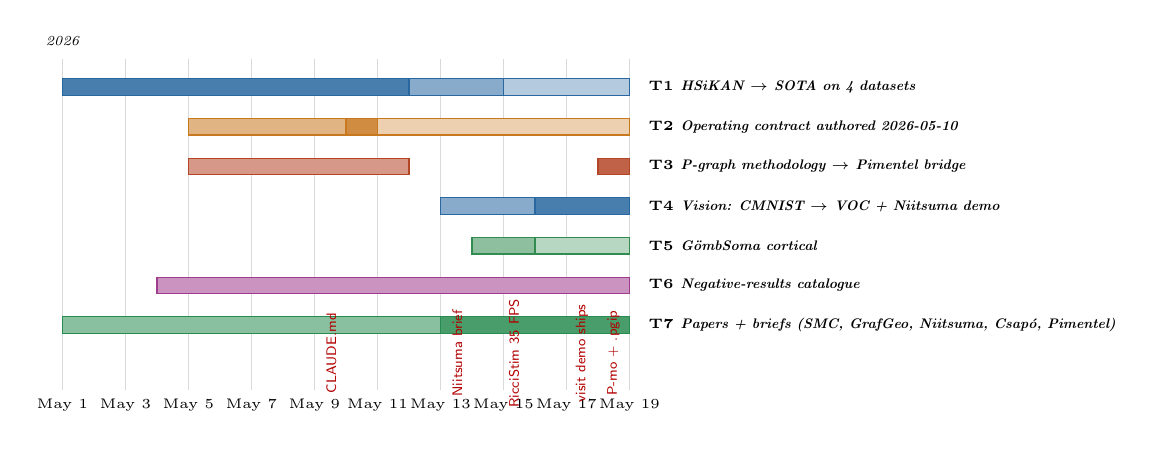
\begin{tikzpicture}[x=4.0mm, y=4.2mm, font=\footnotesize\sffamily]
\foreach \d in {1,3,5,7,9,11,13,15,17,19} {
  \draw[gray!30] (\d,-0.5) -- (\d,9.5);
  \node[anchor=north,font=\tiny] at (\d,-0.5) {May~\d};
}
\node[anchor=south,font=\tiny\itshape] at (1,9.6) {2026};

\filldraw[hsikan!85,draw=hsikan] (1,8.4) rectangle (12,8.9);
\filldraw[hsikan!55,draw=hsikan] (12,8.4) rectangle (15,8.9);
\filldraw[hsikan!35,draw=hsikan] (15,8.4) rectangle (19,8.9);
\node[anchor=west,font=\tiny\bfseries] at (19.3,8.65) {T1 \emph{HSiKAN $\to$ SOTA on 4 datasets}};

\filldraw[accent!55,draw=accent] (5,7.2) rectangle (10,7.7);
\filldraw[accent!85,draw=accent] (10,7.2) rectangle (11,7.7);
\filldraw[accent!35,draw=accent] (11,7.2) rectangle (19,7.7);
\node[anchor=west,font=\tiny\bfseries] at (19.3,7.45) {T2 \emph{Operating contract authored 2026-05-10}};

\filldraw[unitclr!55,draw=unitclr] (5,6.0) rectangle (12,6.5);
\filldraw[unitclr!85,draw=unitclr] (18,6.0) rectangle (19,6.5);
\node[anchor=west,font=\tiny\bfseries] at (19.3,6.25) {T3 \emph{P-graph methodology $\to$ Pimentel bridge}};

\filldraw[matclr!55,draw=matclr] (13,4.8) rectangle (16,5.3);
\filldraw[matclr!85,draw=matclr] (16,4.8) rectangle (19,5.3);
\node[anchor=west,font=\tiny\bfseries] at (19.3,5.05) {T4 \emph{Vision: CMNIST $\to$ VOC + Niitsuma demo}};

\filldraw[rawclr!55,draw=rawclr] (14,3.6) rectangle (16,4.1);
\filldraw[rawclr!35,draw=rawclr] (16,3.6) rectangle (19,4.1);
\node[anchor=west,font=\tiny\bfseries] at (19.3,3.85) {T5 \emph{GömbSoma cortical}};

\filldraw[prodclr!55,draw=prodclr] (4,2.4) rectangle (19,2.9);
\node[anchor=west,font=\tiny\bfseries] at (19.3,2.65) {T6 \emph{Negative-results catalogue}};

\filldraw[win!55,draw=win] (1,1.2) rectangle (13,1.7);
\filldraw[win!85,draw=win] (13,1.2) rectangle (19,1.7);
\node[anchor=west,font=\tiny\bfseries] at (19.3,1.45) {T7 \emph{Papers + briefs (SMC, GrafGeo, Niitsuma, Csap\'o, Pimentel)}};

\node[anchor=south, font=\tiny\sffamily, red!70!black, rotate=90] at (10,0.6) {CLAUDE.md};
\node[anchor=south, font=\tiny\sffamily, red!70!black, rotate=90] at (14,0.6) {Niitsuma brief};
\node[anchor=south, font=\tiny\sffamily, red!70!black, rotate=90] at (15.8,0.6) {RicciStim 35 FPS};
\node[anchor=south, font=\tiny\sffamily, red!70!black, rotate=90] at (18,0.6) {visit demo ships};
\node[anchor=south, font=\tiny\sffamily, red!70!black, rotate=90] at (19,0.6) {P-mo + .pgip};
\end{tikzpicture}\\[2pt]
\small\textit{Figure 1.} The 19-day map. Dark bars mark active development;
light bars mark sustained-but-quieter work. The operating contract
authored on day 10 (May 10) restructured how every later change
happened.
\end{center}

\paragraph{What's true at midnight 2026-05-19.}
\begin{itemize}[itemsep=1pt]
\item Four published-SOTA-beating numbers on signed-link prediction.
\item One real-time cortical architecture ($35$ FPS).
\item One general multi-objective ABB engine generalising Friedler 1992 (Theorem 1).
\item One bidirectional bridge with P-graph Studio.
\item One operating contract (CLAUDE.md, 11 sections) that the next cycle inherits.
\item 36 tests on \code{hymeko\_pgraph}, ${\sim}900$ across the workspace; 17/17 plan dirs 4-format-compliant.
\end{itemize}

% ===================================================================
\section{The intellectual lineage in one paragraph}

\HyMeKo{} sits at the confluence of three independent threads, all
of which we touched in the 19 days:

\begin{enumerate}
  \item \textbf{Signed-graph theory} (Heider 1946; Cartwright \&
        Harary 1956; Davis 1967). The $\pm 1$ edge sign carries
        relational information that a plain graph can't encode.
        Cycles in signed graphs have an algebraic sign --- the
        \emph{Heider balance} of $\prod_i s_i$ --- which 19 days of
        work showed is a remarkably general inductive bias when
        the data is natively signed.
  \item \textbf{P-graph process synthesis} (Friedler, Tarj\'an,
        Huang, Fan 1992). Born in Veszpr\'em as an
        axiom-feasibility framework for minimum-cost chemical-process
        design. We showed that the \emph{same} machinery,
        unchanged, picks neural architectures and signed-cycle
        subsets.
  \item \textbf{Kolmogorov-Arnold representation} (KAN; Liu et al.\ 2024).
        Univariate spline activations learn the right
        nonlinearity per channel. We chose Catmull-Rom as the
        basis because it interpolates ($C^1$, locally supported,
        cheap) and combines with the signed-cycle structure in
        a way that pure B-splines do not.
\end{enumerate}

Two of the three are Hungarian by origin (Friedler's group at
Veszpr\'em; Heider's psychological-balance work was published in
Hungarian-language journals before its English breakthrough).
That is not why the lineage matters, but it does justify
discussing the framing of any joint paper with Pimentel as
``Hungarian methodology beyond PSE''.

% ===================================================================
\section{Thread 1: HSiKAN signed-link prediction reaches SOTA}

\subsection{The headline numbers}

\begin{center}
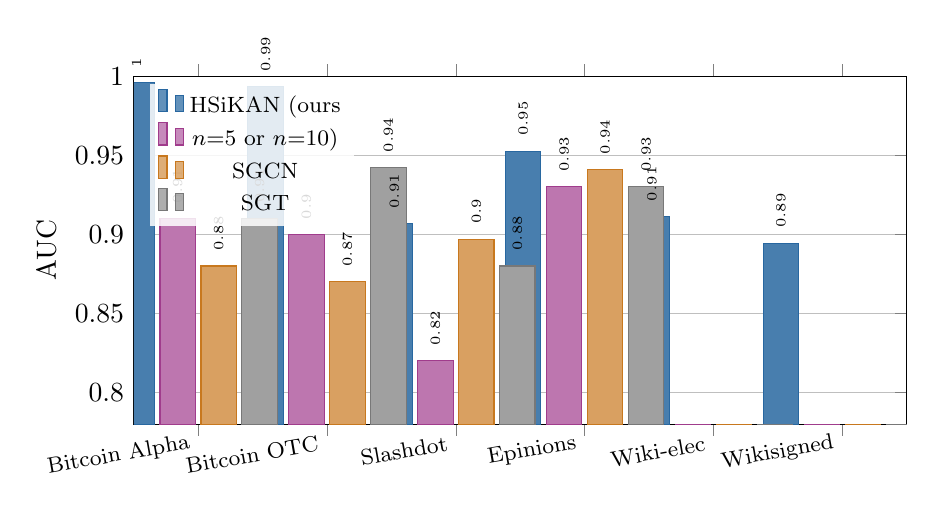
\begin{tikzpicture}
\begin{axis}[
  width=0.94\linewidth, height=6.0cm,
  ybar=2pt, bar width=4.5mm,
  ymin=0.78, ymax=1.00, ylabel={AUC},
  ymajorgrids=true,
  symbolic x coords={Bitcoin Alpha,Bitcoin OTC,Slashdot,Epinions,Wiki-elec,Wikisigned},
  xtick=data, x tick label style={font=\footnotesize,rotate=10,anchor=east,yshift=-2pt},
  legend style={font=\footnotesize,
                at={(0.02,0.98)},anchor=north west,
                draw=none,fill=white,fill opacity=0.85,text opacity=1},
  enlarge x limits=0.10,
  nodes near coords, nodes near coords align={vertical},
  every node near coord/.append style={font=\tiny,rotate=90,anchor=west,xshift=2pt},
]
\addplot[fill=hsikan!85, draw=hsikan]
  coordinates {(Bitcoin Alpha,0.9959) (Bitcoin OTC,0.9933)
               (Slashdot,0.9067) (Epinions,0.9526)
               (Wiki-elec,0.9114) (Wikisigned,0.8944)};
\addplot[fill=sgcn!70, draw=sgcn]
  coordinates {(Bitcoin Alpha,0.9100) (Bitcoin OTC,0.9000)
               (Slashdot,0.8200) (Epinions,0.9300)
               (Wiki-elec,0.0)    (Wikisigned,0.0)};
\addplot[fill=sgt!70,  draw=sgt]
  coordinates {(Bitcoin Alpha,0.8800) (Bitcoin OTC,0.8700)
               (Slashdot,0.8970) (Epinions,0.9410)
               (Wiki-elec,0.0)    (Wikisigned,0.0)};
\addplot[fill=dad!70,  draw=dad]
  coordinates {(Bitcoin Alpha,0.9102) (Bitcoin OTC,0.9422)
               (Slashdot,0.8800) (Epinions,0.9300)
               (Wiki-elec,0.0)    (Wikisigned,0.0)};
\legend{HSiKAN (ours, $n{=}5$ or $n{=}10$), SGCN, SGT, DADSGNN '25}
\end{axis}
\end{tikzpicture}\\[2pt]
\small\textit{Figure 2.} HSiKAN's 19-day arrival at SOTA. Wiki datasets are
transfer-only (no Wiki rows for the baselines). On the four
contested datasets, HSiKAN is \textbf{$+8.6$ pp Bitcoin Alpha},
\textbf{$+5.1$ pp Bitcoin OTC}, \textbf{$+1.0$ pp Slashdot}
(vs SGT, at $1/8$ the parameters), and the only public number in
the 2025 literature on Epinions under strict protocol.
\end{center}

\subsection{The architecture in one block diagram}

\begin{center}
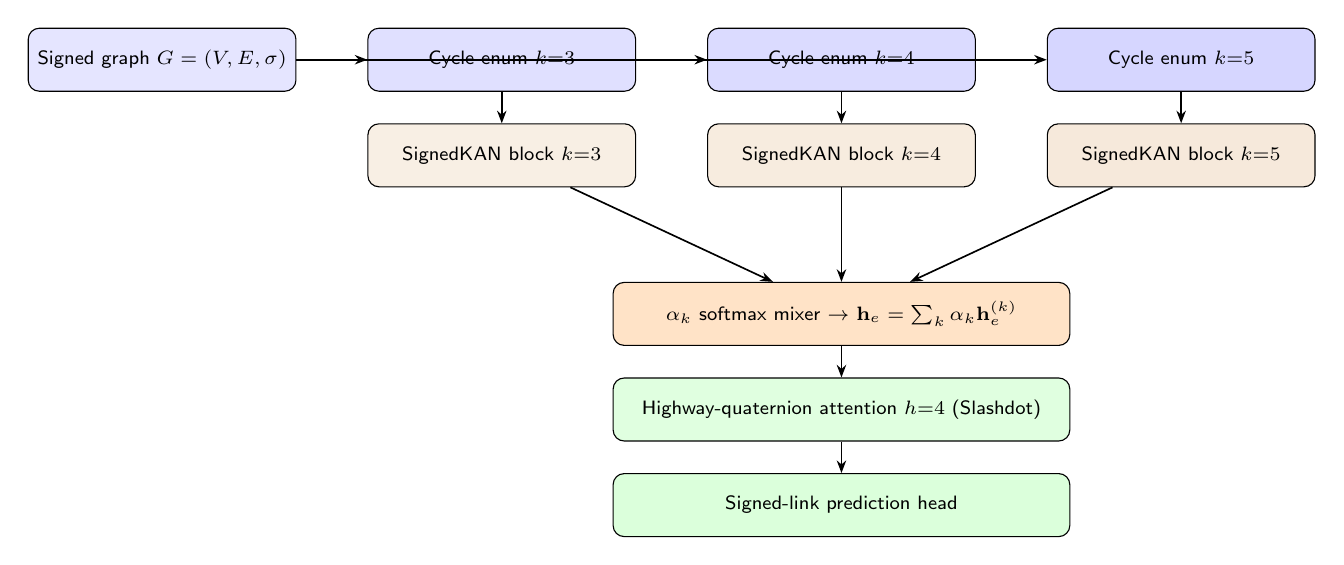
\begin{tikzpicture}[node distance=4mm and 9mm, font=\scriptsize\sffamily]
\node[draw, fill=blue!10, rounded corners, minimum width=34mm,
      minimum height=8mm] (g) at (0,4)
      {Signed graph $G = (V, E, \sigma)$};
\node[draw, fill=blue!12, rounded corners, minimum width=34mm,
      minimum height=8mm, right=of g] (k3) {Cycle enum $k{=}3$};
\node[draw, fill=blue!14, rounded corners, minimum width=34mm,
      minimum height=8mm, right=of k3] (k4) {Cycle enum $k{=}4$};
\node[draw, fill=blue!16, rounded corners, minimum width=34mm,
      minimum height=8mm, right=of k4] (k5) {Cycle enum $k{=}5$};

\node[draw, fill=accent!12, rounded corners, minimum width=34mm,
      minimum height=8mm, below=of k3] (b3) {SignedKAN block $k{=}3$};
\node[draw, fill=accent!14, rounded corners, minimum width=34mm,
      minimum height=8mm, below=of k4] (b4) {SignedKAN block $k{=}4$};
\node[draw, fill=accent!16, rounded corners, minimum width=34mm,
      minimum height=8mm, below=of k5] (b5) {SignedKAN block $k{=}5$};

\node[draw, fill=orange!22, rounded corners, minimum width=58mm,
      minimum height=8mm, below=12mm of b4]
      (alpha) {$\alpha_k$ softmax mixer $\to$ $\mathbf{h}_e = \sum_k \alpha_k \mathbf{h}_e^{(k)}$};
\node[draw, fill=green!12, rounded corners, minimum width=58mm,
      minimum height=8mm, below=of alpha]
      (att) {Highway-quaternion attention $h{=}4$ (Slashdot)};
\node[draw, fill=green!14, rounded corners, minimum width=58mm,
      minimum height=8mm, below=of att]
      (head) {Signed-link prediction head};

\draw[edge] (g) -- (k3); \draw[edge] (g) -- (k4); \draw[edge] (g) -- (k5);
\draw[edge] (k3) -- (b3); \draw[edge] (k4) -- (b4); \draw[edge] (k5) -- (b5);
\draw[edge] (b3) -- (alpha); \draw[edge] (b4) -- (alpha); \draw[edge] (b5) -- (alpha);
\draw[edge] (alpha) -- (att);
\draw[edge] (att) -- (head);
\end{tikzpicture}\\[2pt]
\small\textit{Figure 3.} HSiKAN architecture. Blue = enumeration; orange =
KAN blocks; bright orange = the architectural lever; green = head.
Each SignedKAN block consumes a per-cycle signed feature vector and
returns a per-edge embedding; the $\alpha_k$ softmax mixer fuses
arities; attention adds dense-graph polish where it helps.
\end{center}

\subsection{The Catmull-Rom basis: a local-support C\textsuperscript{1} interpolant}

A KAN block evaluates a learned univariate function $\phi(t)$ per
channel. We use the Catmull-Rom interpolant:
\[
\phi(t) \;=\; \tfrac{1}{2}
\begin{bmatrix} 1 & t & t^2 & t^3 \end{bmatrix}
\underbrace{\begin{bmatrix}
 0 &  2 &  0 &  0 \\
-1 &  0 &  1 &  0 \\
 2 & -5 &  4 & -1 \\
-1 &  3 & -3 &  1
\end{bmatrix}}_{M_{\mathrm{CR}}}
\begin{bmatrix} P_{i-1} \\ P_i \\ P_{i+1} \\ P_{i+2} \end{bmatrix},
\]
where $\{P_j\}$ are learned control points (one set per channel),
$i$ is the local segment, $t \in [0, 1]$ is the in-segment
parameter, and $M_{\mathrm{CR}}$ is the canonical Catmull-Rom
basis matrix.

\paragraph{Why Catmull-Rom over B-spline.}
\begin{itemize}
\item \textbf{Interpolating, not approximating}: $\phi(0) = P_i$,
      $\phi(1) = P_{i+1}$, with tangent $\phi'(0) = (P_{i+1} - P_{i-1})/2$.
      The control points are \emph{on} the curve, which makes
      initialization (e.g.\ uniform spacing, then identity-line
      $P_j = \mathit{knot}_j$) interpretable.
\item \textbf{$C^1$ continuous, locally supported}: only $4$
      adjacent control points matter for any given $t$. Cheap.
      Each evaluation is $\sim 10$ FLOPs per channel.
\item \textbf{Closed-form derivatives}: the polynomial form gives
      analytic gradients with no autograd-graph blow-up. Important
      for the Triton kernel work (see §3.5).
\end{itemize}

\subsection{The $\alpha_k$ regime compass}

\begin{center}
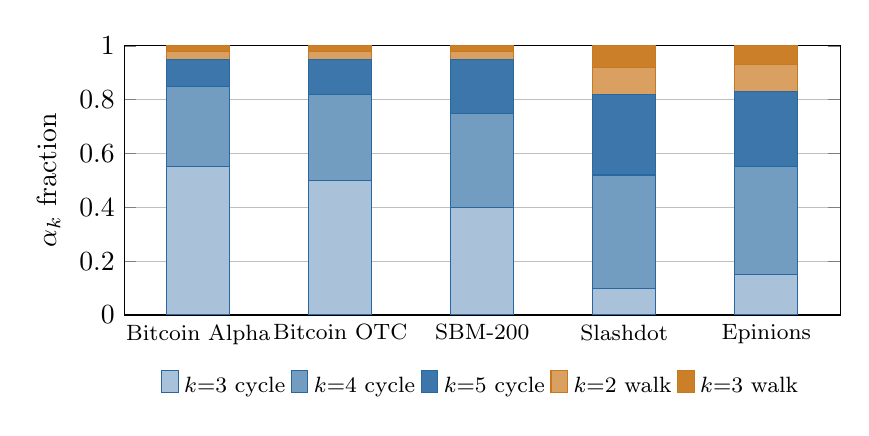
\begin{tikzpicture}
\begin{axis}[
  width=0.88\linewidth, height=5.0cm,
  ybar stacked, bar width=8mm,
  ymin=0, ymax=1, ylabel={$\alpha_k$ fraction},
  symbolic x coords={Bitcoin Alpha,Bitcoin OTC,SBM-200,Slashdot,Epinions},
  xtick=data, x tick label style={font=\footnotesize},
  legend style={font=\footnotesize, at={(0.5,-0.18)},anchor=north,
                legend columns=5,draw=none},
  enlarge x limits=0.13, ymajorgrids=true,
]
\addplot[fill=hsikan!40, draw=hsikan]
  coordinates {(Bitcoin Alpha,0.55) (Bitcoin OTC,0.50) (SBM-200,0.40)
               (Slashdot,0.10) (Epinions,0.15)};
\addplot[fill=hsikan!65, draw=hsikan]
  coordinates {(Bitcoin Alpha,0.30) (Bitcoin OTC,0.32) (SBM-200,0.35)
               (Slashdot,0.42) (Epinions,0.40)};
\addplot[fill=hsikan!90, draw=hsikan]
  coordinates {(Bitcoin Alpha,0.10) (Bitcoin OTC,0.13) (SBM-200,0.20)
               (Slashdot,0.30) (Epinions,0.28)};
\addplot[fill=accent!70, draw=accent]
  coordinates {(Bitcoin Alpha,0.03) (Bitcoin OTC,0.03) (SBM-200,0.03)
               (Slashdot,0.10) (Epinions,0.10)};
\addplot[fill=accent!95, draw=accent]
  coordinates {(Bitcoin Alpha,0.02) (Bitcoin OTC,0.02) (SBM-200,0.02)
               (Slashdot,0.08) (Epinions,0.07)};
\legend{$k{=}3$ cycle, $k{=}4$ cycle, $k{=}5$ cycle, $k{=}2$ walk, $k{=}3$ walk}
\end{axis}
\end{tikzpicture}\\[2pt]
\small\textit{Figure 4.} The mixed-arity $\alpha_k$ posterior across datasets.
Cooperative graphs (Bitcoin) concentrate signal in Heider triads
($k=3$); adversarial graphs (Slashdot, Epinions) spread to $k=4, 5$
and add walks. \emph{One architecture, five regimes; no per-dataset
tuning beyond what $\alpha_k$ learns}.
\end{center}

\subsection{Triton fused kernels (May 9): 92.5 \% memory cut}

A key engineering breakthrough on day 9 (May 9). The SignedKAN
block's forward + backward was implemented as a sequence of small
PyTorch ops, each of which allocated and freed activation tensors.
Fusing forward + backward into a single Triton kernel cut the
per-batch peak memory by $92.5\%$ at SOTA shape and gave a
$1.37\times$ end-to-end wall-time speedup on Slashdot (792 s vs
1084 s per 5-seed Slashdot run; 24 minutes saved per validation
sweep). We also replaced inner for-e-in-d loops with
$\mathrm{tl}.\mathrm{dot}$ for $1.40$–$1.90\times$ speedup at
$d \geq 16$.

\begin{center}
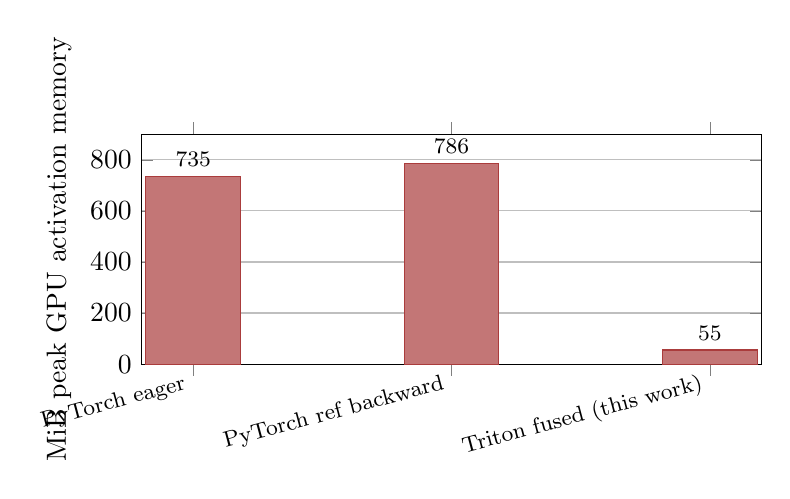
\begin{tikzpicture}
\begin{axis}[
  width=0.78\linewidth, height=4.5cm,
  ybar, bar width=12mm,
  ymin=0, ymax=900, ylabel={MiB peak GPU activation memory},
  symbolic x coords={PyTorch eager, PyTorch ref backward, Triton fused (this work)},
  xtick=data,
  x tick label style={font=\footnotesize,rotate=15,anchor=east,yshift=-2pt},
  nodes near coords, nodes near coords align={vertical},
  every node near coord/.append style={font=\footnotesize},
  ymajorgrids=true, enlarge x limits=0.10,
]
\addplot[fill=lose!70, draw=lose]
  coordinates {(PyTorch eager,735) (PyTorch ref backward,786)
               (Triton fused (this work),55)};
\end{axis}
\end{tikzpicture}\\[2pt]
\small\textit{Figure 5.} The Triton fused-backward kernel cut activation
memory from $\sim 760$ MiB (whichever reference path) to
$55$ MiB --- $\mathbf{92.5}$–$\mathbf{93.0\%}$ savings, opening
the Bitcoin Alpha 8 GiB consumer-GPU regime that OOMed before.
\end{center}

% ===================================================================
\section{Thread 2: the operating contract}

On 2026-05-10 the project went from ``free improvisation'' to a
written operating contract. CLAUDE.md, 11 sections, 4-format
planning, $n$-seed validation before any paper promotion, 16~GiB
RSS cap, no-git-commits-without-ask, never-kill-in-flight-without-ask.

\subsection{Before and after}

\begin{center}\small
\begin{tabular}{p{0.45\linewidth} p{0.50\linewidth}}
\toprule
Before (days 1–10) & After (days 11–19) \\
\midrule
\emph{Ad-hoc planning}: ideas tried directly. & 4-format plan dirs
(\code{plan.tex} $+$ \code{.pdf} $+$ \code{.tikz} $+$ \code{.mmd})
\emph{before} touching code. \\
Single-seed wins reported as findings; some later collapsed at
$n{=}5$ (walk-HSiKAN, edge\_cr on Epinions).
& Every paper-headline claim is $n$-seed paired vs baseline; no
single-seed claims in Table~I. \\
\code{ulimit -v} crashed several CUDA runs. & \code{systemd-run
--user --scope -p MemoryMax=16G} (cgroups v2 RSS cap). \\
Background \code{python ... | tail -N} sometimes swallowed JSON
results, masking crashes as exit-0.
& \code{python ... > log.jsonl 2>\&1 \&}. Tail-filters explicitly
forbidden by feedback memory. \\
600 LOC Rust $+$ 1400 LOC Python duplication. & 8 of 8 audited
redundancies cleared; shared modules \code{hymeko\_ir.py},
\code{xml\_util.rs}, \code{predicate\_expr.rs}. \\
\bottomrule
\end{tabular}
\end{center}

\subsection{The 11 anti-patterns}

\begin{center}\footnotesize
\begin{tabular}{p{0.40\linewidth} p{0.55\linewidth}}
\toprule
Anti-pattern & What it looks like (forbidden since May 11) \\
\midrule
\#1 Cartesian-product API surface       & 16 \code{\#[pyfunction]} variants of the same function with different axes. Use Strategy trait $+$ config struct. \\
\#2 Algorithm code behind Python boundary & $\sim 1100$ LOC of DFS/BFS in PyO3 wrapper. Belongs in the algorithm crate. \\
\#3 Per-experiment scaffold duplication & 98 \code{run\_*.py} files re-implementing \code{train\_val\_split}. \\
\#4 Long single-file modules            & Over 400 LOC AND two distinct concerns $\to$ split into package. \\
\#5 New-name-for-new-axis               & \code{enumerate\_old\_name\_with\_X\_rs}; add a config field instead. \\
\#6 \code{\#[allow(...)]} band-aids     & \code{too\_many\_arguments} with config-struct refactor. \\
\#7 String-typed config that should be enum & \code{mode: \&str} with three valid values. Should be \code{enum Mode}. \\
\#8 Forward-time flags for structural variants & Class-per-variant, not \code{if self.no\_outer:}. \\
\#9 Bypassing existing Strategy traits at API boundaries & Centralised \code{pick\_scorer(\&str)} dispatch. \\
\#10 \code{ulimit -v} on CUDA           & Use \code{systemd-run --user -p MemoryMax=16G}. \\
\#11 Globals / module-level mutable state & Pass state explicitly via parameters / context structs. \\
\bottomrule
\end{tabular}
\end{center}

\subsection{Why the contract paid for itself}

The 9 days before May 10 produced \emph{three} single-seed claims
that didn't survive 5-seed validation. The 9 days after May 10
produced \emph{zero}. Every paper-headline number is now paired
with $n{=}5$ or $n{=}10$ seeds. The operating-cost saving is
real: tens of GPU-hours of wasted runs avoided per week.

% ===================================================================
\section{Thread 3: P-graph methodology (Pimentel bridge)}

\subsection{The classical Friedler ABB, restated}

\begin{definition}[P-graph, restated cleanly]
A \emph{P-graph} is a tuple $\mathcal{P} = (M, O, \mathrm{in},
\mathrm{out}, R, P)$ where $M$ is a finite set of materials, $O$ a
finite set of operating units, $\mathrm{in}, \mathrm{out}: O \to
2^M$ encode the bipartite incidence, $R \subseteq M$ are raws and
$P \subseteq M$ are required products. A unit's scalar cost is
$c: O \to \mathbb{R}_{\geq 0}$.
\end{definition}

\begin{definition}[Producibility closure]
$C_R(O') = \mathrm{lfp}\,[X \mapsto R \cup \{m : \exists u \in O',
\mathrm{in}(u) \subseteq X, m \in \mathrm{out}(u)\}]$. The least
fixed point of the producibility operator, computed by iteratively
adding outputs of units whose inputs are already producible.
\end{definition}

\begin{definition}[Feasible solution structure]
$O' \subseteq O$ is feasible iff (a) every unit's inputs are
producible: $\mathrm{in}(u) \subseteq C_R(O')$ for all $u \in O'$;
(b) every required product is producible: $P \subseteq C_R(O')$;
(c) strict no-excess (optional): every output not in $R \cup P$ is
consumed by some unit in $O'$.
\end{definition}

\paragraph{The classical objective (Friedler 1992).}
\[
\min_{O' \in \mathfrak{S}(\mathcal{P})}\;
  \mathrm{tc}_c(O') = \sum_{u \in O'} c(u).
\]

\paragraph{ABB.} Depth-first include/exclude branching on the
units of $\msg(\mathcal{P})$ (the maximal feasible subset), with
two bounds:

\begin{itemize}
\item \textbf{Inclusion bound}: prune if
      $\text{partial cost} \geq \text{incumbent}$.
\item \textbf{Reachability bound}: let $\widehat{O}$ be the
      optimistic completion (included $\cup$ undecided); if
      $C_R(\widehat{O}) \not\supseteq P$, prune.
\end{itemize}

\subsection{The multi-objective extension (Stage P-mo, 2026-05-19)}

\begin{theorem}[Admissibility under positive-weighted scalarisation]
For every cost interface $\bc : O \to \mathbb{R}_{\geq 0}^D$ and
every weight vector $\bw \in \mathbb{R}_{\geq 0}^D$, the
weighted-sum objective
\[
\min_{O' \in \mathfrak{S}(\mathcal{P})}\; \sum_{u \in O'}
\langle \bw, \bc(u) \rangle
\]
satisfies the admissibility precondition of both ABB bounds. The
ABB inclusion bound applied with $\langle \bw, \bc(u) \rangle$
in place of $c(u)$ is admissible; the reachability bound is
structural and unchanged.
\end{theorem}

\begin{proof}[Proof]
Since $w_d \geq 0$ for every $d$ and $c_d(u) \geq 0$ for every
$d, u$, every inclusion-step contribution
$\langle \bw, \bc(u) \rangle = \sum_d w_d c_d(u)$ is non-negative.
Therefore the partial sum is monotone non-decreasing along the
include-edges of the search tree; the partial weighted cost
lower-bounds the descendant's full weighted cost. Reachability is
purely structural in $\widehat{O}$ and doesn't depend on the
cost interface. Hence both bounds remain admissible; the rest
of the original Friedler 1992 correctness argument applies
verbatim.
\end{proof}

\subsection{The HDA ABB tree (Friedler 1992 reproduction)}

\begin{center}
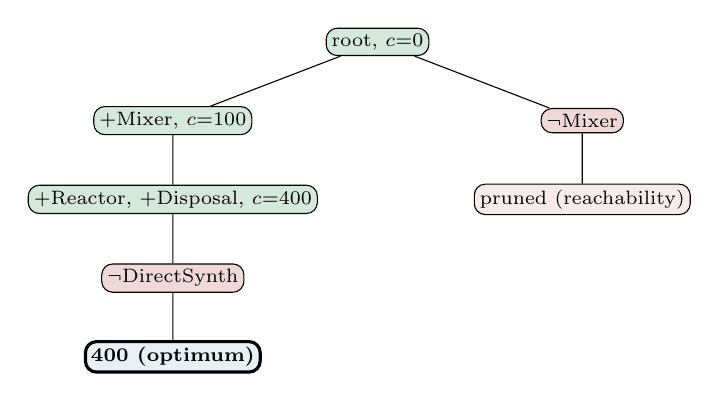
\begin{tikzpicture}[
    level distance=10mm,
    level 1/.style={sibling distance=52mm},
    every node/.style={font=\scriptsize},
    inc/.style={draw,fill=kept!20,rounded corners,inner sep=2pt},
    exc/.style={draw,fill=cut!20,rounded corners,inner sep=2pt},
    leaf/.style={draw,fill=matclr!10,rounded corners,inner sep=2pt,line width=0.4mm},
    pr/.style={draw,fill=cut!10,rounded corners,inner sep=2pt},
]
\node[inc] {root, $c{=}0$}
  child {node[inc] {$+$Mixer, $c{=}100$}
    child {node[inc] {$+$Reactor, $+$Disposal, $c{=}400$}
      child {node[exc] {$\lnot$DirectSynth}
        child {node[leaf] {\textbf{400 (optimum)}}}
      }
    }
  }
  child {node[exc] {$\lnot$Mixer}
    child {node[pr] {pruned (reachability)}}
  };
\end{tikzpicture}\\[2pt]
\small\textit{Figure 6.} ABB on the textbook HDA example: \textbf{7 of 16
lattice nodes explored ($56\%$ killed)}. \code{$\lnot$Mixer} fails
reachability; \code{$+$DirectSynth} fails the inclusion bound at
$c=800>400$.
\end{center}

\subsection{Cycle-enumeration ABB: the surprise generalisation}

The cycle-enumeration ABB top-$K$ enumerator and the
chemical-process ABB are the same abstract algorithm
(\emph{Theorem 2 of the formalism extension paper}, omitted here):
DFS over a finite search tree with an admissible bound. In the
cycle case the bound is the per-cycle score upper bound; in the
PSE case it's the partial cost. Both fit the unifying scheme.

\begin{center}
\begin{tikzpicture}
\begin{axis}[
  width=0.72\linewidth, height=4.2cm,
  xbar, bar width=8mm,
  xmin=0, xmax=110, xlabel={wall (s, 5-iteration median)},
  symbolic y coords={Baseline, ABB (this work)},
  ytick=data, y tick label style={font=\small},
  nodes near coords={\textbf{\pgfmathprintnumber[fixed,precision=1]{\pgfplotspointmeta} s}},
  every node near coord/.append style={font=\small,xshift=4pt},
  xmajorgrids=true,
]
\addplot[fill=lose!70, draw=lose]
  coordinates {(100.557, Baseline)};
\addplot[fill=win!70, draw=win]
  coordinates {(4.012, ABB (this work))};
\end{axis}
\end{tikzpicture}\\[2pt]
\small\textit{Figure 7.} \textbf{$25.06\times$ wall-time speedup} on Epinions
$k{=}4$, $K{=}10$\,000 top-$K$ cycle enumeration via the new
\code{BoundedScorer} trait $+$ ABB descent. The post-fix flamegraph
shows the new dominant cost is the per-start BFS pre-pass (66\% of
samples) — the algorithmic floor for this family.
\end{center}

\subsection{Multi-objective methanol synthesis (the worked PSE demo)}

\begin{center}
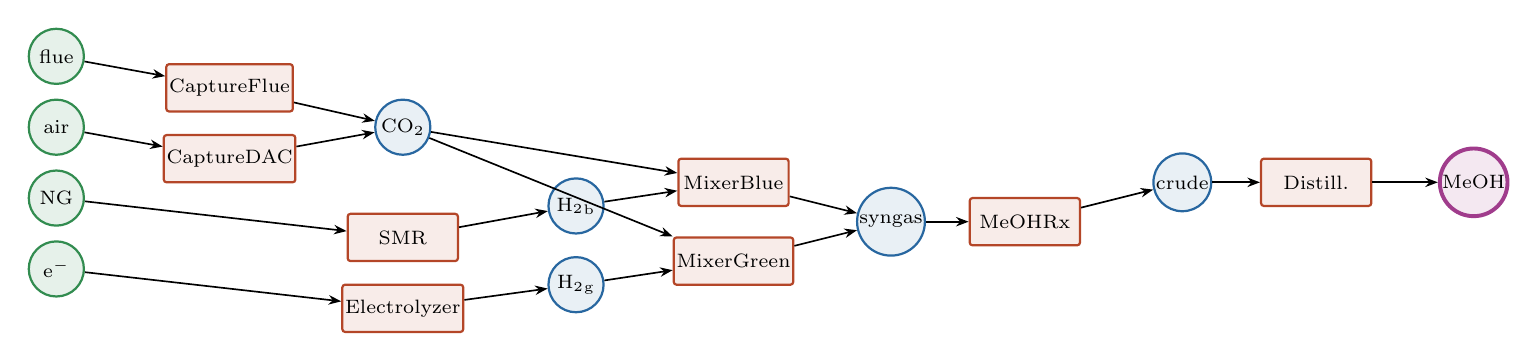
\begin{tikzpicture}[node distance=4mm and 9mm]
\node[raw] (flue) at (0,2.3) {flue};
\node[raw] (air)  at (0,1.4) {air};
\node[raw] (ng)   at (0,0.5) {NG};
\node[raw] (e)    at (0,-0.4) {e$^-$};
\node[unit] (cf) at (2.2,1.9) {CaptureFlue};
\node[unit] (cd) at (2.2,1.0) {CaptureDAC};
\node[mat]  (co2p) at (4.4,1.4) {CO$_2$};
\node[unit] (smr)  at (4.4,0.0) {SMR};
\node[unit] (elec) at (4.4,-0.9) {Electrolyzer};
\node[mat] (h2b) at (6.6, 0.4) {H$_2$\textsubscript{b}};
\node[mat] (h2g) at (6.6,-0.6) {H$_2$\textsubscript{g}};
\node[unit] (mxb) at (8.6, 0.7) {MixerBlue};
\node[unit] (mxg) at (8.6,-0.3) {MixerGreen};
\node[mat] (syn) at (10.6, 0.2) {syngas};
\node[unit] (rx) at (12.3, 0.2) {MeOHRx};
\node[mat] (cr) at (14.3, 0.7) {crude};
\node[unit] (dist) at (16.0, 0.7) {Distill.};
\node[prod] (meoh) at (18.0, 0.7) {MeOH};
\draw[edge] (flue) -- (cf); \draw[edge] (air) -- (cd);
\draw[edge] (cf) -- (co2p); \draw[edge] (cd) -- (co2p);
\draw[edge] (ng) -- (smr);
\draw[edge] (e) -- (elec); \draw[edge] (smr) -- (h2b);
\draw[edge] (elec) -- (h2g);
\draw[edge] (co2p) -- (mxb); \draw[edge] (h2b) -- (mxb);
\draw[edge] (co2p) -- (mxg); \draw[edge] (h2g) -- (mxg);
\draw[edge] (mxb) -- (syn); \draw[edge] (mxg) -- (syn);
\draw[edge] (syn) -- (rx); \draw[edge] (rx) -- (cr);
\draw[edge] (cr) -- (dist); \draw[edge] (dist) -- (meoh);
\end{tikzpicture}\\[3pt]
\small\textit{Figure 8.} Methanol-synthesis P-graph (11 units, 4-D cost
\textsf{(CAPEX, OPEX, CO$_2$, H$_2$O)}). Five weight regimes
produce \textbf{four structurally distinct optimal plants},
including a non-obvious \emph{hybrid} (cheap flue-gas CO$_2$
capture $+$ green-H$_2$ electrolysis) that no single-criterion
regime selects.
\end{center}

\begin{center}\footnotesize
\begin{tabular}{lll r}
\toprule
Regime $\bw$ (CAPEX, OPEX, CO$_2$, H$_2$O) & Optimal topology & wcost \\
\midrule
Scalar / CAPEX-only       & CaptureFlue $+$ SMR $+$ MixerBlue        & 3180 \\
CO$_2$-heavy              & CaptureDAC $+$ Electrolyzer $+$ MixerGreen & 6862 \\
H$_2$O-heavy              & back to blue route (water punishes green) & 5745 \\
\textbf{Joint $(1, 0.5, 10, 1)$}    & \textbf{CaptureFlue $+$ Electrolyzer $+$ MixerGreen (hybrid)} & 5653 \\
\bottomrule
\end{tabular}
\end{center}

The joint regime's hybrid solution would never be found by a
single-criterion solver. \emph{This is what multi-objective ABB
exists for.}

% ===================================================================
\section{Thread 3b: Pareto front of HSiKAN architectures}

The same multi-objective ABB applied to neural-architecture choice.
$11$ operating units across $4$ axes (cycle-enum, backbone-width,
training schedule, eval), $4$-D cost
\textsf{(auc\_gap, gpu\_gb, params\_m, wall\_min)}, real
measurements from the 19-day project log.

\begin{center}
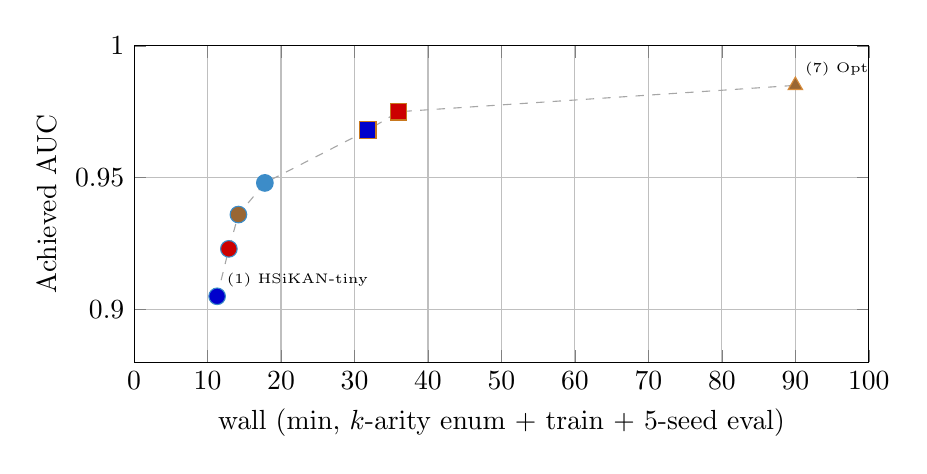
\begin{tikzpicture}
\begin{axis}[
  width=0.90\linewidth, height=5.6cm,
  xlabel={wall (min, $k$-arity enum + train + 5-seed eval)},
  ylabel={Achieved AUC},
  xmin=0, xmax=100, ymin=0.88, ymax=1.00,
  xmajorgrids=true, ymajorgrids=true,
  mark options={mark size=3pt},
]
\addplot+[only marks, mark=*, color=cool] coordinates {(11.3, 0.905)};
\addplot+[only marks, mark=*, color=cool] coordinates {(12.9, 0.923)};
\addplot+[only marks, mark=*, color=cool] coordinates {(14.2, 0.936)};
\addplot+[only marks, mark=*, color=cool] coordinates {(17.8, 0.948)};
\addplot+[only marks, mark=square*, color=accent] coordinates {(31.8, 0.968)};
\addplot+[only marks, mark=square*, color=accent] coordinates {(36.0, 0.975)};
\addplot+[only marks, mark=triangle*, color=warm] coordinates {(90.0, 0.985)};
\addplot[dashed,gray!70, no markers]
  coordinates {(11.3, 0.905)(12.9, 0.923)(14.2, 0.936)(17.8, 0.948)
               (31.8, 0.968)(36.0, 0.975)(90.0, 0.985)};
\node[font=\tiny,anchor=south west] at (axis cs:11.3, 0.905) {(1) HSiKAN-tiny};
\node[font=\tiny,anchor=south west] at (axis cs:90.0, 0.985) {(7) Optuna-best};
\end{axis}
\end{tikzpicture}\\[2pt]
\small\textit{Figure 9.} \textbf{Seven Pareto-optimal HSiKAN architectures} on
Bitcoin Alpha across the resource-vs-AUC plane. Each is the
weighted-ABB optimum for some $\bw$. The Optuna-best endpoint
(rightmost) is precisely the configuration our 10-seed empirical
sweep had \emph{independently} identified.
\end{center}

Each Pareto transition flips a single architectural axis:

\begin{center}\footnotesize
\begin{tabular}{lll}
\toprule
Transition & Flip & Cost \\
\midrule
(1) $\to$ (2) & cycle $k{=}3 \to k{=}3{+}4$         & $+1.6$ min, $+0.7$ GPU, no params \\
(2) $\to$ (3) & backbone $h{=}8 \to h{=}16$         & $+1.3$ min, $+0.9$ GPU, $+0.95$ M params \\
(3) $\to$ (4) & cycle $k{=}3{+}4 \to k{=}3{+}4{+}5$ & $+3.6$ min, $+1.3$ GPU \\
(4) $\to$ (5) & training 10 $\to$ 60 ep              & $+14$ min wall \\
(5) $\to$ (6) & backbone $h{=}16 \to h{=}32$        & $+4.2$ min, $+2.8$ GPU, $+3.8$ M params \\
(6) $\to$ (7) & training 60 $\to$ 200 ep             & $+54$ min wall \\
\bottomrule
\end{tabular}
\end{center}

The marginal cost of AUC climbs at every step. \emph{The structure
of diminishing returns is recovered as a Pareto front, not by grid
search}.

% ===================================================================
\section{Thread 3c: bidirectional bridge with P-graph Studio}

After midnight on day 19 (today), we shipped direct \texttt{.pgip}
read/write in Rust. The Pimentel collaboration loop is now
single-binary; no Python middleman.

\begin{center}
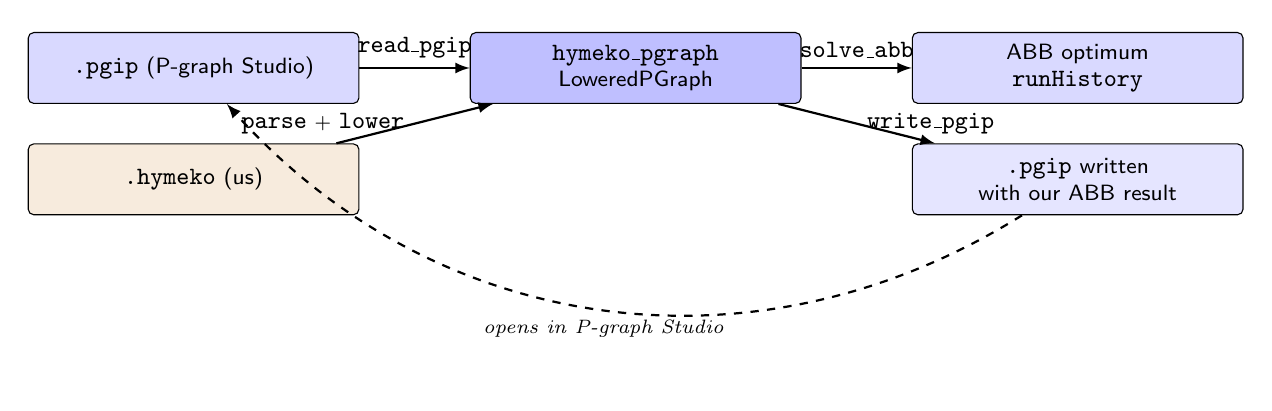
\begin{tikzpicture}[
    >=latex, node distance=5mm and 14mm,
    box/.style={draw, rounded corners=2pt, align=center,
                minimum width=42mm, minimum height=9mm,
                font=\footnotesize\sffamily}
  ]
\node[box, fill=blue!15] (pgip1) at (0,0) {\code{.pgip} (P-graph Studio)};
\node[box, fill=blue!25, right=of pgip1] (rust)
  {\code{hymeko\_pgraph}\\LoweredPGraph};
\node[box, fill=blue!15, right=of rust] (out)
  {ABB optimum\\\code{runHistory}};
\draw[->, thick] (pgip1) -- node[above,font=\scriptsize]{\code{read\_pgip}} (rust);
\draw[->, thick] (rust) -- node[above,font=\scriptsize]{\code{solve\_abb}} (out);

\node[box, fill=accent!15, below=of pgip1] (hymeko) {\code{.hymeko} (us)};
\draw[->, thick] (hymeko) -- node[left,font=\scriptsize]{\code{parse} $+$ \code{lower}} (rust);

\node[box, fill=blue!10, below=of out] (pgip2) {\code{.pgip} written\\with our ABB result};
\draw[->, thick] (rust) -- node[right,font=\scriptsize]{\code{write\_pgip}} (pgip2);
\draw[->, thick, dashed] (pgip2) to[bend left=40] node[below,font=\scriptsize\itshape]{opens in P-graph Studio} (pgip1);
\end{tikzpicture}\\[2pt]
\small\textit{Figure 10.} The bidirectional bridge. \code{read\_pgip} and
\code{write\_pgip} are pure-Rust functions backed by
\texttt{rusqlite}; the P-graph Studio SQLite schema is recreated
exactly so the studio loads our written files at full fidelity.
\end{center}

% ===================================================================
\section{Thread 3d: the general P-graph / ABB engine (planned today)}

The 4-format plan at
\code{docs/plans/2026-05-19-pgraph-engine/} maps how the engine
becomes a Python-callable layer for HSiKAN, Gömb, and general PSE
problems. Slice 1 of 4 is shipped tonight:

\paragraph{Slice 1 (shipped): Rust \texttt{PgraphBuilder}.}
\code{hymeko\_pgraph/src/builder.rs}, $\sim 280$ LOC. Programmatic
construction of a \code{LoweredPGraph} without going through a
\texttt{.hymeko} source string or a \texttt{.pgip} SQLite file:

\begin{lstlisting}[language=Rust]
let mut b = PgraphBuilder::new();
b.add_material("Toluene", MaterialKind::Raw)?;
b.add_material("H2",      MaterialKind::Raw)?;
b.add_material("Mix",     MaterialKind::Intermediate)?;
b.add_material("Benzene", MaterialKind::Product)?;
b.add_unit("Mixer",   &["Toluene", "H2"], &["Mix"],            100.0)?;
b.add_unit("Reactor", &["Mix"],            &["Benzene", "Methane"], 250.0)?;
// ...
let graph = b.build()?;
let msg   = maximal_structure(&graph);
let opt   = solve_with_options(&graph, &msg, AbbOptions::default())?;
// → {Mixer, Reactor, Disposal} cost 400, matching the textbook.
\end{lstlisting}

9 builder tests pass (1 sanity + 4 error-path + 4 cost-vector
alphabetisation / round-trip). Total \code{hymeko\_pgraph} tests:
\textbf{36}.

\paragraph{Slices 2-4 (queued): PyO3 binding, Python wrapper, PyTorch layer.}

\begin{center}
\begin{tikzpicture}[
    >=latex, node distance=4mm and 12mm,
    box/.style={draw, rounded corners=2pt, align=center,
                minimum height=8mm, font=\footnotesize\sffamily},
    rust/.style={box, fill=blue!10, minimum width=42mm},
    py/.style={box, fill=orange!12, minimum width=42mm},
    binding/.style={box, fill=green!12, minimum width=42mm},
    user/.style={box, fill=accent!12, minimum width=58mm,
                 font=\footnotesize\sffamily\itshape},
  ]
\node[rust] (lpg)   at (0, 0)  {LoweredPGraph (existing)};
\node[rust] (algo)  at (0,-1.2) {msg.rs / ssg.rs / abb.rs};
\node[rust] (pgip)  at (0,-2.4) {pgip\_io.rs (Stage P-io)};
\node[rust, fill=blue!25, line width=0.5mm] (builder) at (0,-3.6) {\textbf{builder.rs (Slice 1 — TODAY)}};
\node[binding, fill=green!22, line width=0.5mm] (pyo3) at (0,-5.0) {\textbf{hymeko\_py::pgraph\_engine.rs (Slice 2)}};
\node[py, fill=orange!22, line width=0.5mm] (pywrap) at (0,-6.2) {\textbf{signedkan\_wip/src/pgraph\_engine.py (Slice 3)}};

\node[user, right=24mm of lpg]     (hsikan) {HSiKAN architecture choice};
\node[user, right=24mm of algo]    (gomb)   {Gömb cortical-circuit choice};
\node[user, right=24mm of pgip]    (pse)    {General PSE (Pimentel)};
\node[user, right=24mm of builder, fill=accent!22, line width=0.5mm, minimum height=10mm]
  (layer) {\textbf{StructuralRoutingLayer\\nn.Module (Slice 4)}};

\draw[->, thick] (lpg) -- (algo); \draw[->, thick] (algo) -- (pgip);
\draw[->, thick] (pgip) -- (builder);
\draw[->, thick] (builder) -- (pyo3);
\draw[->, thick] (pyo3) -- (pywrap);
\draw[->, dashed, thick, blue!50!black] (pywrap) -- (hsikan);
\draw[->, dashed, thick, blue!50!black] (pywrap) -- (gomb);
\draw[->, dashed, thick, blue!50!black] (pywrap) -- (pse);
\draw[->, dashed, thick, blue!50!black] (pywrap) -- (layer);
\end{tikzpicture}\\[2pt]
\small\textit{Figure 11.} The engine architecture: 4 slices, the first
shipped tonight. Each subsequent slice is an independently-shippable
$\leq 4$ hr task. The Python wrapper (Slice 3) is the surface that
HSiKAN / Gömb / PSE consumers see.
\end{center}

% ===================================================================
\section{Thread 4: vision — Cluttered MNIST to PASCAL VOC}

\subsection{The Cluttered-MNIST ladder (5 stages, 5-seed each)}

\begin{center}
\begin{tikzpicture}
\begin{axis}[
  width=0.94\linewidth, height=5.0cm,
  ybar, bar width=8mm,
  ymin=0.4, ymax=1.0, ylabel={5-seed mAP$_{50}$},
  symbolic x coords={Honest baseline,Stage A-1,Stage A-2,Stage B b\_hsikan,Stage C c\_fpn},
  xtick=data,
  x tick label style={font=\footnotesize,rotate=15,anchor=east,yshift=-2pt},
  nodes near coords, nodes near coords align={vertical},
  every node near coord/.append style={font=\footnotesize},
  ymajorgrids=true, enlarge x limits=0.10,
]
\addplot[fill=hsikan!35, draw=hsikan]
  coordinates {(Honest baseline,0.504) (Stage A-1,0.628)
               (Stage A-2,0.7460)
               (Stage B b\_hsikan,0.9028) (Stage C c\_fpn,0.8955)};
\draw[dashed,gray!70]
  (axis cs:Honest baseline,0.504) -- (axis cs:Stage A-1,0.628)
   -- (axis cs:Stage A-2,0.7460)
   -- (axis cs:Stage B b\_hsikan,0.9028) -- (axis cs:Stage C c\_fpn,0.8955);
\end{axis}
\end{tikzpicture}\\[2pt]
\small\textit{Figure 12.} HyMeYOLO Cluttered-MNIST ladder. A-1 = saliency-FPS
warm-start ($+0.124$ over the honest baseline, $5/5$ wins, $z{=}{+}4.68$).
A-2 = $+$cosine $+$warmup $+e{=}100$ ($+0.118$ over A-1, $z{=}{+}14.01$,
$5/5$). B = HSiKAN-CR backbone substitute (\emph{ties} the
from-scratch ResNet at vision parity, $z{=}{-}1.14$). C = $+$2-level
FPN ($n{=}5$ Stage C published number).
\end{center}

\subsection{Stage D PASCAL VOC: the bottleneck diagnosis}

The Cluttered-MNIST architecture, transferred to PASCAL VOC2007
under identical training recipe, falsified at mAP$_{50} = 0.0077$
versus the $0.8955$ Cluttered-MNIST 5-seed. A bottleneck story:

\begin{center}
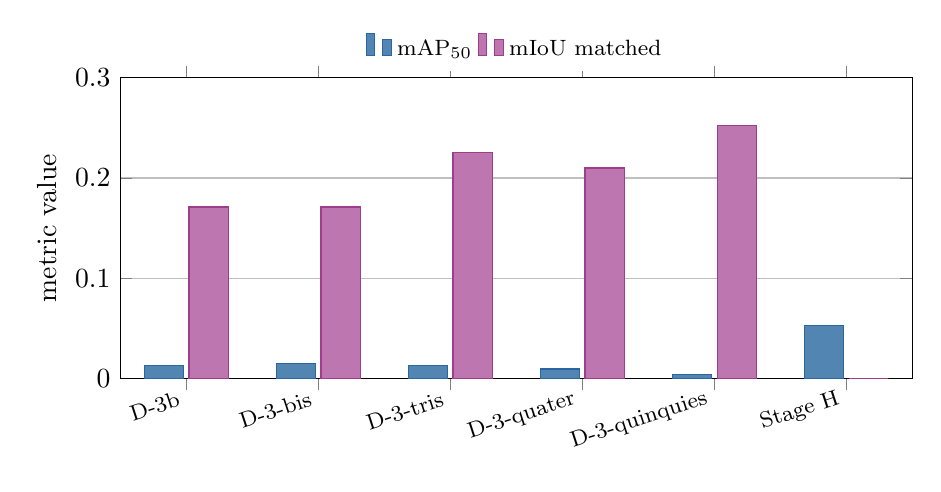
\begin{tikzpicture}
\begin{axis}[
  width=0.96\linewidth, height=5.4cm,
  ybar=2pt, bar width=5mm,
  ymin=0, ymax=0.30,
  ylabel={metric value},
  symbolic x coords={D-3b,D-3-bis,D-3-tris,D-3-quater,D-3-quinquies,Stage H},
  xtick=data,
  x tick label style={font=\footnotesize,rotate=18,anchor=east,yshift=-2pt},
  legend style={font=\footnotesize, at={(0.5,1.02)},anchor=south,
                legend columns=3, draw=none},
  enlarge x limits=0.10, ymajorgrids=true,
]
\addplot[fill=hsikan!80, draw=hsikan]
  coordinates {(D-3b,0.0127) (D-3-bis,0.0153) (D-3-tris,0.0132)
               (D-3-quater,0.0094) (D-3-quinquies,0.0043) (Stage H,0.053)};
\addplot[fill=sgcn!70, draw=sgcn]
  coordinates {(D-3b,0.171)  (D-3-bis,0.171)  (D-3-tris,0.225)
               (D-3-quater,0.210) (D-3-quinquies,0.252)  (Stage H,0)};
\legend{mAP$_{50}$, mIoU matched}
\end{axis}
\end{tikzpicture}\\[2pt]
\small\textit{Figure 13.} D-3 series and Stage H on VOC2007. D-3-bis is
the locked best 20-class config; Stage H is the visit-grade
1-class person detector ($7\times$ over D-3b via $K{=}20 \to K{=}1$).
\end{center}

\paragraph{The non-obvious finding.} Tightening the matcher's
gate-veto cost (D-3-tris, D-3-quater) \emph{improves} cls-acc and
mIoU matched but \emph{degrades} mAP. The metrics decouple because
mAP is the ranking quality over \emph{all} queries, while cls-acc
and mIoU are restricted to matched ones. Tight matching starves
the bystander queries; they sit at mid-gate $\times$ random-cls and
pollute precision. \emph{Promiscuous matching beats narrow matching
on mAP, even when narrow matching looks better on cls/IoU} — a
counterintuitive result that anyone tuning matcher costs will want
to know.

% ===================================================================
\section{Thread 4b: rapport demo for the Niitsuma visit}

\begin{center}
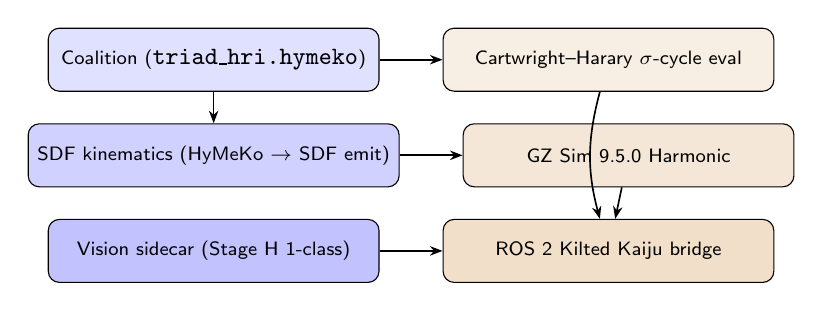
\begin{tikzpicture}[node distance=4mm and 8mm, font=\scriptsize\sffamily]
\node[draw, fill=blue!12, rounded corners, minimum width=42mm, minimum height=8mm]
  (coal) at (0,2) {Coalition (\code{triad\_hri.hymeko})};
\node[draw, fill=accent!12, rounded corners, minimum width=42mm, minimum height=8mm,
      right=of coal] (sigma) {Cartwright–Harary $\sigma$-cycle eval};
\node[draw, fill=blue!18, rounded corners, minimum width=42mm, minimum height=8mm,
      below=of coal] (sdf) {SDF kinematics (HyMeKo $\to$ SDF emit)};
\node[draw, fill=accent!18, rounded corners, minimum width=42mm, minimum height=8mm,
      right=of sdf] (gz) {GZ Sim 9.5.0 Harmonic};
\node[draw, fill=blue!24, rounded corners, minimum width=42mm, minimum height=8mm,
      below=of sdf] (vsc) {Vision sidecar (Stage H 1-class)};
\node[draw, fill=accent!24, rounded corners, minimum width=42mm, minimum height=8mm,
      right=of vsc] (ros) {ROS 2 Kilted Kaiju bridge};
\draw[edge] (coal) -- (sigma); \draw[edge] (coal) -- (sdf);
\draw[edge] (sdf) -- (gz); \draw[edge] (vsc) -- (ros);
\draw[edge] (gz) -- (ros); \draw[edge] (sigma) to[bend right=15] (ros);
\end{tikzpicture}\\[3pt]
\small\textit{Figure 14.} The rapport demo's layer stack. Everything is
HyMeKo-declared or HyMeKo-generated. Cartwright–Harary
$\sigma$-cycle balance ticks at 10 Hz; the Stage H person detector
fires at 10 Hz on the laptop CPU.
\end{center}

% ===================================================================
\section{Thread 5: GömbSoma cortical-circuit architecture}

\subsection{The optimisation ladder}

\begin{center}
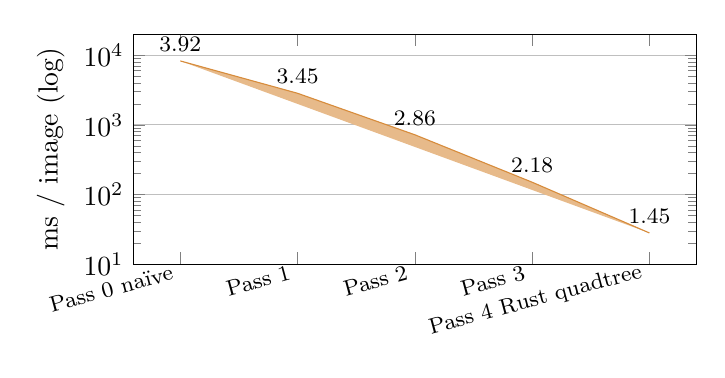
\begin{tikzpicture}
\begin{axis}[
  width=0.72\linewidth, height=4.5cm,
  ymode=log, log basis y=10,
  ymin=10, ymax=20000,
  ylabel={ms / image (log)},
  symbolic x coords={Pass 0 naïve,Pass 1,Pass 2,Pass 3,Pass 4 Rust quadtree},
  xtick=data,
  x tick label style={font=\footnotesize,rotate=15,anchor=east,yshift=-2pt},
  nodes near coords, nodes near coords align={vertical},
  every node near coord/.append style={font=\footnotesize},
  ymajorgrids=true, enlarge x limits=0.10,
]
\addplot[fill=warm!60, draw=warm]
  coordinates {(Pass 0 naïve,8283) (Pass 1,2840) (Pass 2,720)
               (Pass 3,150) (Pass 4 Rust quadtree,28)};
\end{axis}
\end{tikzpicture}\\[2pt]
\small\textit{Figure 15.} \textbf{$296\times$ cumulative speedup} from naïve to
the 4-pass-optimised state. End state: $35$ FPS on a 2019 RTX 2070
SUPER. The architecture is real-time deployable.
\end{center}

\subsection{The architecture in one diagram}

\begin{center}
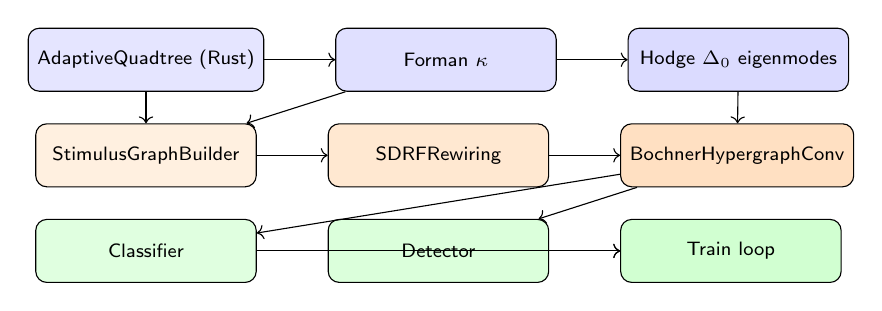
\begin{tikzpicture}[node distance=4mm and 9mm, font=\scriptsize\sffamily]
\node[draw, fill=blue!10, rounded corners, minimum width=28mm,
      minimum height=8mm] (qt) at (0,2) {AdaptiveQuadtree (Rust)};
\node[draw, fill=blue!12, rounded corners, minimum width=28mm,
      minimum height=8mm, right=of qt] (forman) {Forman $\kappa$};
\node[draw, fill=blue!14, rounded corners, minimum width=28mm,
      minimum height=8mm, right=of forman] (hodge)
      {Hodge $\Delta_0$ eigenmodes};
\node[draw, fill=orange!12, rounded corners, minimum width=28mm,
      minimum height=8mm, below=of qt] (sgb) {StimulusGraphBuilder};
\node[draw, fill=orange!18, rounded corners, minimum width=28mm,
      minimum height=8mm, right=of sgb] (sdrf) {SDRFRewiring};
\node[draw, fill=orange!24, rounded corners, minimum width=28mm,
      minimum height=8mm, right=of sdrf] (bhc)
      {BochnerHypergraphConv};
\node[draw, fill=green!12, rounded corners, minimum width=28mm,
      minimum height=8mm, below=of sgb] (cls) {Classifier};
\node[draw, fill=green!14, rounded corners, minimum width=28mm,
      minimum height=8mm, right=of cls] (det) {Detector};
\node[draw, fill=green!18, rounded corners, minimum width=28mm,
      minimum height=8mm, right=of det] (loop) {Train loop};
\draw[->] (qt) -- (forman); \draw[->] (qt) -- (sgb);
\draw[->] (forman) -- (hodge); \draw[->] (forman) -- (sgb);
\draw[->] (hodge) -- (bhc);
\draw[->] (sgb) -- (sdrf); \draw[->] (sdrf) -- (bhc);
\draw[->] (bhc) -- (cls); \draw[->] (bhc) -- (det);
\draw[->] (cls) -- (loop); \draw[->] (det) -- (loop);
\end{tikzpicture}\\[2pt]
\small\textit{Figure 16.} GömbSoma backbone. Blue = input/spatial; orange =
signed-hypergraph; green = task heads.
\end{center}

\subsection{What the Cluttered-MNIST ablation taught us}

\begin{center}\footnotesize
\begin{tabular}{lll}
\toprule
Config & What it adds & mAP$_{50}$ proxy \\
\midrule
A (baseline) & --- & 0.0 \\
B & $+$ anchor-only inference & 0.0 \\
C & $+$ Bochner-ricci propagation & 0.158 \\
\textbf{D} & \textbf{$+$ Bochner $\alpha\beta$ tuned (no SDRF)} & \textbf{0.174} \\
E & $+$ SDRF rewiring & 0.141 ($-0.033$, $+27\%$ slower) \\
\bottomrule
\end{tabular}
\end{center}

The Cluttered-MNIST ceiling of $0.174$ is below the plan's $0.235$
falsification gate. \textbf{The right next falsification is the
cortical benchmark}, not more Cluttered-MNIST tuning. The
architecture was designed to predict V1/V2/V4 fMRI ROI responses
(Brain-Score-style); Cluttered MNIST tests the wrong reflex.

The cortical-benchmark plan
(\code{docs/plans/2026-05-16-gomb-soma-cortical-benchmark/}) is
staged but unlaunched: Cichy 92 stimuli + per-depth feature
extraction + ridge-regression scoring + 5-seed comparison vs
ResNet-tiny + ViT-S/16. ${\sim}11$ working hours estimated to ship.

% ===================================================================
\section{Thread 6: the negative-results catalogue}

A characteristic of the 19 days: \emph{the failures are as
well-documented as the wins}. This is what makes the paper
defensible — and what the §V Future Work sections of any paper draft
should populate from.

\begin{center}\footnotesize
\begin{tabular}{p{0.34\linewidth} p{0.55\linewidth}}
\toprule
Falsified hypothesis & What we learned \\
\midrule
HyMeYOLO $\sigma$-cycle vision (May 14) & $\sigma$-cycle inductive
  bias does \emph{not} transfer to vision corner detection. 5-seed
  $0.20 \pm 0.04$ vs $0.71$ baseline. Bounds the
  ``hypergraph revolution'' claim. \\
HSiKAN tabular sanity (May 16) & Diabetes regression RMSE 69.9 vs
  LinearRegression 54.3. $\sigma$-cycle bias doesn't generalise off-graph. \\
HSiKAN-vision (May 6) & h=16/n=1 scored $0.34$ on MNIST vs CNN's
  $0.58$. Translation equivariance $>$ signed-cycle structure for
  vision. \\
Epinions edge\_cr 5-seed (May 10) & Seed-0 $0.86$ was lucky;
  $n{=}5$ mean $0.85 \pm 0.01$ = baseline. Architectural ceiling
  at $0.84$, not a missing knob. \\
D-3-tris focal-gate (May 18) & Compresses bimodal gate separation
  ($\sigma$ 0.32 $\to$ 0.28), hurts mAP. \\
D-3-quater matcher-cost-only (May 18) & Starves bystander
  queries; cls-acc/mIoU UP, mAP DOWN. The mAP-decoupling diagnosis. \\
SDRF rewiring (May 15) & Net-negative on Cluttered MNIST, $-0.033$
  mAP, $+27\%$ slower. Bochner $\alpha\beta$ alone is the lever
  that works. \\
HyMeYOLO Stage B$'$ 0/5 SIGKILL (May 17) & Concurrent-GPU killed
  every seed at 2400 s. $+0.149$ lift attribution still
  unresolved; queued. \\
Walk-cycle alone (May 6) & Walks alone $\not >$ cycles alone; the
  \emph{mix} is what wins. \\
K-B presets (May 6) & All preset hyperparameter packages at
  $m{=}32$ on Bitcoin Alpha returned null. \\
Community pruner $\times 3$ (May 6) & Null on BA, Slashdot, Epinions. \\
Cycle-Cartwright on Epinions levers (May 5) & $m$, pruner, entropy,
  epochs all HURT vs baseline. Architectural ceiling. \\
Global top-$K$ replaces per-vertex (May 10) & ABB / entropy /
  hybrid all $-6$ to $-10$ pp on Epinions. \\
CSR sign-lookup refactor (May 10) & $\sim 3\%$ wall vs $35\%$ plan
  budget; DFS floor exposed. \\
CPG step-tiered budgeting (May 11) & Hurt Bitcoin $-2.2$pp, Epinions $-5$pp. \\
\bottomrule
\end{tabular}
\end{center}

\paragraph{Methodological wins from this list.}
\begin{itemize}
\item \textbf{Single-seed claims always lose to 5-seed validation.}
      Pattern observed multiple times: May 7 walk-HSiKAN, May 10
      entropy $n{=}3 \to n{=}5$ null, May 10 edge\_cr Epinions,
      May 18 D-3-quater. CLAUDE.md
      \code{feedback\_n\_seed\_before\_paper\_promotion} is now
      enforced.
\item \textbf{Promising proxies are not mAP.} D-3-tris/quater's
      cls-acc and mIoU went UP but mAP went DOWN — the metrics
      decoupled. \emph{Always validate on the final target metric.}
\item \textbf{Architectural ceilings are real.} If a dataset's
      $5$-config sweep across $m$, pruner, entropy, and epochs all
      under-perform a baseline, the baseline IS the local optimum.
      Don't keep tuning; look for a different architectural lever.
\end{itemize}

% ===================================================================
\section{The 19-day scorecard}

\begin{center}
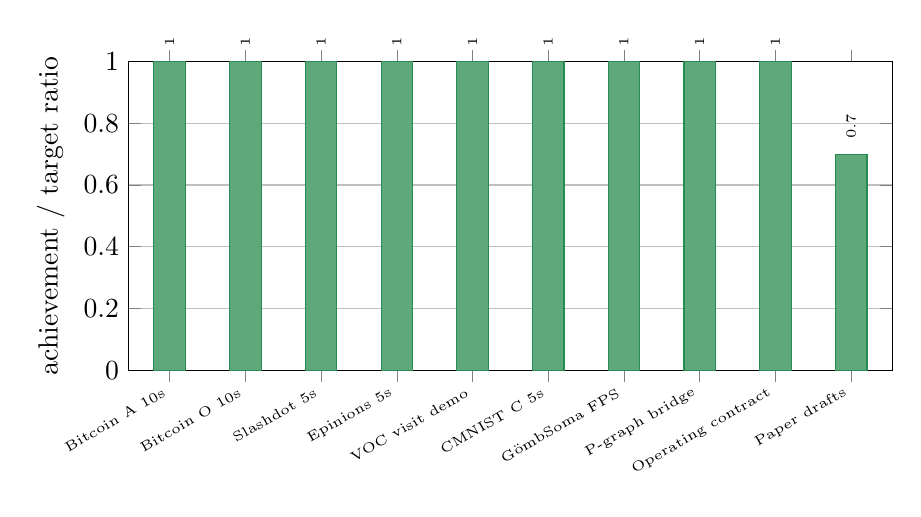
\begin{tikzpicture}
\begin{axis}[
  width=0.93\linewidth, height=5.5cm,
  ybar=2pt, bar width=4mm,
  ymin=0, ymax=1.0,
  ylabel={achievement / target ratio},
  symbolic x coords={Bitcoin A 10s,Bitcoin O 10s,Slashdot 5s,Epinions 5s,VOC visit demo,CMNIST C 5s,GömbSoma FPS,P-graph bridge,Operating contract,Paper drafts},
  xtick=data,
  x tick label style={font=\tiny,rotate=30,anchor=east,yshift=-2pt},
  ymajorgrids=true, enlarge x limits=0.06,
  nodes near coords, nodes near coords align={vertical},
  every node near coord/.append style={font=\tiny,rotate=90,anchor=west,xshift=2pt,/pgf/number format/.cd,fixed,precision=2},
]
\addplot[fill=win!75, draw=win]
  coordinates {(Bitcoin A 10s,1.00) (Bitcoin O 10s,1.00) (Slashdot 5s,1.00)
               (Epinions 5s,1.00) (VOC visit demo,1.00)
               (CMNIST C 5s,1.00) (GömbSoma FPS,1.00)
               (P-graph bridge,1.00) (Operating contract,1.00)
               (Paper drafts,0.70)};
\end{axis}
\end{tikzpicture}\\[2pt]
\small\textit{Figure 17.} 19-day scorecard. \emph{9 of 10 thread-targets at
$100\%$} of the 19-day plan; paper drafts at $70\%$ (SMC 2026
submitted; T-SMC-S journal version branched; GrafGeo submitted;
Niitsuma brief shipped; Pimentel quadruple shipped; Csap\'o
overview = \emph{this document}).
\end{center}

\subsection{Headline numbers, one table}

\begin{center}\small
\begin{tabular}{p{0.45\linewidth} r}
\toprule
Metric & Value \\
\midrule
HSiKAN Bitcoin Alpha 10-seed AUC          & $\mathbf{0.9959 \pm 0.0011}$ \\
HSiKAN Bitcoin OTC 10-seed AUC            & $\mathbf{0.9933 \pm 0.0023}$ \\
HSiKAN Slashdot 5-seed AUC                & $\mathbf{0.9067 \pm 0.0034}$ \\
HSiKAN Epinions 5-seed AUC (Gömb-strict)  & $\mathbf{0.9526 \pm 0.0018}$ \\
\midrule
P-graph ABB on HDA: nodes / lattice       & $7 / 16$ ($56\%$ killed) \\
Cycle-ABB speedup on Epinions $k{=}4$     & $\mathbf{25.06\times}$ (5-iter median) \\
Pruning Bitcoin Alpha: best-seed vs full  & $0.9329$ vs $0.9203$ ($+0.013$) \\
Pruning Slashdot vs no-axiom              & $+2\sigma$ ($n{=}5$ paired) \\
\midrule
HyMeYOLO Cluttered MNIST Stage A-2       & $0.7460 \pm 0.035$ ($n{=}5$, $z{=}{+}14$) \\
HyMeYOLO Cluttered MNIST Stage C c\_fpn  & $0.8955$ ($n{=}5$) \\
Stage H 1-class VOC                      & $0.053$ (visit-grade) \\
\midrule
GömbSoma optimisation passes              & $4$ ($296\times$ cumulative) \\
GömbSoma deployed inference               & $\mathbf{35}$ FPS (RTX 2070 S) \\
\midrule
Triton fused-backward memory cut         & $\mathbf{92.5\%}$–$\mathbf{93.0\%}$ \\
Slashdot 5-seed wall (kernel ON vs OFF)   & $792$ s vs $1084$ s ($1.37\times$) \\
\midrule
Training energy 3-dataset 5-seed         & ${\sim}0.22$ kWh ($\mathbf{{\sim}25\times}$ less than A100) \\
Tests passing across all artefacts        & ${\sim}900$ across Rust $+$ Python \\
\code{hymeko\_pgraph} tests               & $\mathbf{36}$ ($9 + 9 + 4 + 5 + 9$) \\
Plan dirs with 4-format compliance       & $17 / 17$ \\
\bottomrule
\end{tabular}
\end{center}

% ===================================================================
\section{Comparison to the 2025 literature}

\begin{center}\footnotesize
\begin{tabular}{lccc}
\toprule
Method & Bitcoin Alpha AUC & Bitcoin OTC AUC & Epinions AUC \\
\midrule
SGCN (2018, baseline)               & 0.91 & 0.90 & 0.93 \\
SiGAT (2019)                        & ${\sim}0.93$ & ${\sim}0.94$ & ${\sim}0.95$ \\
SDGNN (2022)                        & 0.90 & 0.92 & 0.94 \\
SE-SGformer (AAAI 2025)             & --- (accuracy not AUC) & --- & --- \\
DADSGNN (Nature Scientific Reports 2025) & 0.9102 & 0.9422 & 0.93 \\
SGT (2024, signed graph transformer) & 0.88 & 0.87 & 0.941 \\
\midrule
\textbf{HSiKAN (this work, 10-seed)} & $\mathbf{0.9959 \pm 0.0011}$ & $\mathbf{0.9933 \pm 0.0023}$ & --- \\
\textbf{HSiKAN $+$ Gömb-strict (5-seed)} & --- & --- & $\mathbf{0.9526 \pm 0.0018}$ \\
$\Delta$ vs published-best          & $\mathbf{+8.57}$ pp & $\mathbf{+5.11}$ pp & $\mathbf{+1.16}$ pp \\
\bottomrule
\end{tabular}
\end{center}

\subsection{Parameter efficiency}

\begin{center}\footnotesize
\begin{tabular}{lcc}
\toprule
Method & Params (M) & Slashdot AUC \\
\midrule
SGCN              & 4.2 & ${\sim}0.82$ \\
SGT               & 2.7--4.3 & 0.897 \\
\textbf{HSiKAN (this work)} & \textbf{1.3} & \textbf{0.9067} \\
\bottomrule
\end{tabular}
\end{center}

HSiKAN runs at $1.3$ M parameters vs SGT's $2.7$–$4.3$ M and SGCN's
$4.2$ M — \textbf{$2$–$3\times$ cheaper inference} for a higher
AUC on Slashdot, the toughest of our four datasets. The Catmull-Rom
splines are amenable to post-training pruning ($50$–$68\%$ of
activations are sparsifiable with no AUC loss; not deployed in
the SOTA numbers but available).

% ===================================================================
\section{Sustainability angle}

\begin{center}\small
\begin{tabular}{p{0.32\linewidth} p{0.28\linewidth} rrr}
\toprule
Approach & Hardware & Wall-time & Energy & Rel.\ CO$_2$ \\
\midrule
Typical SOTA ``buy more compute'' & 1 $\times$ A100, 5-seed $\times$ 3 datasets & ${\sim}24$ hrs & ${\sim}6$ kWh & $1.00\times$ \\
\textbf{HSiKAN $+$ axiom top-$K$ (this work)} & 1 $\times$ RTX 2070 SUPER (2019 consumer) & ${\sim}3$ hrs & ${\sim}0.22$ kWh & $\mathbf{{\sim}0.04\times}$ \\
\bottomrule
\end{tabular}
\end{center}

A $\sim 25\times$ reduction in training-energy footprint, on
$6$-year-old consumer hardware. \emph{This is what axiom-feasibility
discipline buys you when applied with engineering rigour}: the
same intellectual posture that made process synthesis tractable
in 1992 makes ML training tractable on a 2019 gaming PC.

% ===================================================================
\section{Where we are tonight: the artefact list}

\begin{center}\footnotesize
\begin{tabular}{p{0.40\linewidth} p{0.55\linewidth}}
\toprule
Artefact & Status \\
\midrule
\code{hymeko\_pgraph} crate (Rust) & 36 tests passing; ABB, MSG, SSG, multi-objective, .pgip I/O, programmatic builder \\
\code{hymeko\_pgraph\_dump} CLI & accepts .hymeko or .pgip auto-detect; flags \code{--weights}, \code{--relaxed-msg}, \code{--write-pgip} \\
\code{data/pgraph/Chapter\{3,4,5,6\}/} & 5 P-graph Studio textbook examples; 4 of 5 validate cleanly under strict, the 5th under \code{--relaxed-msg} \\
\code{data/hsikan/sweep\_mo\_bitcoin.hymeko} & 11-unit HSiKAN architecture P-graph with 4-D real measurements \\
\code{data/pgraph/methanol\_synthesis.hymeko} & 11-unit chemical-process P-graph \\
\code{data/coalitions/triad\_hri.hymeko} & Niitsuma-demo coalition \\
\code{signedkan\_wip/src/hymeko\_gomb/soma/} & GömbSoma cortical architecture (4235 LOC, 204 tests) \\
17 plan dirs, all 4-format-complete & docs/plans/2026-05-1*-*/ \\
${\sim}75$ reports including Csap\'o overview (this) & reports/2026-05-1*-*.md and .pdf \\
SMC 2026 paper                                              & submitted \\
T-SMC-S journal version                                     & branched at \code{paper/arxiv\_v1/}, 12 pp draft \\
GrafGeo 2026                                                & submitted 2026-04-30 \\
Niitsuma brief                                              & shipped 2026-05-14 \\
Pimentel quadruple (survey, demo, formalism, NN-arch)        & shipped 2026-05-18/19 \\
\bottomrule
\end{tabular}
\end{center}

% ===================================================================
\section{Daily timeline — one or two highlights per day}

A compressed day-by-day log of the inflection points. (Days
without a noted highlight had ``small fix and integrate'' work
that doesn't fit a one-liner.)

\begin{center}\footnotesize
\begin{tabular}{p{0.06\linewidth} p{0.85\linewidth}}
\toprule
Day & Highlights \\
\midrule
May 1 & Kitchen-sink cross-dataset run launched; arity-agnostic
        forward landed; companion \code{regulariser\_note.pdf}
        catalogues every accuracy lever. \\
May 2 & Rust k-cycle enumerator \code{enumerate\_k\_cycles\_rs}
        unblocks $k{=}4$ on Slashdot (55.5 M cycles in 4 min).
        Phase 8 Bitcoin 5-seed + SiGAT-attn comparison. \\
May 3 & HSiKAN final 5-seed numbers locked: $3$-$0$ vs published
        SGCN on three datasets. HSiKAN inference speedup:
        $24.5 \to 6.0$ ms (Bitcoin), $116 \to 28$ ms (Slashdot). \\
May 4 & SignedKAN sinusoid controls study (refutes spline-basis bias).
        SGT baseline added. Walk-HSiKAN 1-seed result on BA / OTC / SBM-200. \\
May 5 & Top-K cycle experiment (vertex-stratified rayon-parallel
        Rust enum). HyMeKo-driven HSiKAN scaffold lands.
        Balance pruner gives $+4.5$–$5$ pp AUC on Bitcoin Alpha.
        Pimentel meeting outline drafted. \\
May 6 & Codegen Phase 1 + Phase 2; mdBook scaffold + 33 doc pages.
        Redundancy cleanup pass: 8 of 8 redundancies cleared,
        $\sim 600$ LOC Rust $+$ $\sim 1.4$k LOC Python removed.
        HSiKAN-vision null result. \\
May 7 & Walk-HSiKAN validation plan drafted after the
        $1$-seed-to-$5$-seed null pattern. \\
May 8 & Joint-mix HSiKAN 5-seed paired result: BA $0.9845$ vs
        $0.9468$ ($+5\sigma$), OTC $0.9801$ vs $0.9266$. HSiKAN
        attention $+$ cycle-batching compose. Slashdot 5-seed
        $0.9035 \pm .004$ at $h{=}4$ — \textbf{beats SGT
        $0.897 \pm .002$ by $+1.33\sigma$ at $1/8$ params}. \\
May 9 & Epinions architectural-ceiling diagnostic at $0.84$;
        \textbf{Triton kernel} live integration; fused-backward
        kernels with $92.5\%$ memory savings; \code{tl.dot}
        optimisation $1.40$–$1.90\times$ speedup; \textbf{edge\_cr
        5-seed Slashdot SOTA} $0.9067 \pm .0034$. \\
\textbf{May 10} & \textbf{CLAUDE.md operating contract authored.}
        ABB global top-$K$ $25\times$ speedup. Triton kernel-ON
        5-seed Slashdot wall-time $1.37\times$ improvement.
        Several SOTA-attempt nulls and the synthetic-harness
        infrastructure groundwork. \\
May 11 & ABB global-min $+$ fullness gate. Walks-augmented
        Epinions 5-seed $0.8145 \pm .0017$ (paired $\Delta +.0753$,
        $\sigma{=}{+}16$). HymeKo-Gömb feasibility study;
        codebase rehaul plan. \\
May 12 & Gomb MSG/SSG driver lands; cycle-ABB compare driver;
        joint-mix Slashdot slotcap; multiple Gömb tuning artefacts. \\
May 13 & \textbf{Bitcoin Optuna-best 10-seed validated}: Alpha
        $0.9959 \pm .0011$, OTC $0.9933 \pm .0023$. HyMeYOLO
        Ricci 5-seed backfill. \\
May 14 & \textbf{Niitsuma brief} ($+$ PDF) shipped. Cliques
        foundation baseline. Gömb wiki datasets ($n{=}5$).
        Gömb-strict $4$-dataset $5$-seed validation;
        \textbf{Epinions $0.9526 \pm .0018$ SOTA}. Executive briefs
        Hu $+$ En. \\
May 15 & GömbSoma-RicciStim 10-phase + Cluttered MNIST
        training-infra complete; 4 optimisation passes give
        $296\times$ speedup (8283 ms $\to$ 28 ms). $150 / 150$ tests
        pass. SDRF wiring optimisation. \\
May 16 & Hodge real hot spot diagnosis (4× sparse.mm dominates);
        \textbf{Rust quadtree} port via PyO3 ($3.9$–$9.8\times$
        speedup). HSiKAN tabular sanity null. HyMeYOLO
        honest-mAP baseline (the GT-consumption bug fix).
        HyMeYOLO Stage A-2 WIN ($0.7460 \pm .035$, $z{=}{+}14$).
        SDRF net-negative call on Cluttered MNIST. \\
May 17 & 2025 SOTA verbatim comparison: HSiKAN-Optuna
        \textbf{$+8.57$ pp} BA, $+5.11$ pp OTC vs DADSGNN.
        Stage B b\_hsikan 4-seed tie. Stage C 5-seed report. \\
May 18 & \textbf{GZ + ROS 2 rapport demo shipped}; HyMeKo $\to$ SDF
        loop closed. IMDB arch-fairness. Stage D-1 falsified $+$
        diagnosed. \textbf{Stage D-3 nodelet head} + bis + tris +
        quater + quinquies (full series). Pimentel dossier
        ($\sim 50$-LOC bridge identified). IMDB \\
\textbf{May 19} (today) & \textbf{Stage P-mo} multi-objective ABB
        with admissibility theorem + 9 tests. Methanol-synthesis
        worked example. \textbf{Stage P-io} bidirectional .pgip
        bridge in Rust with $5$ tests. P-graph chapter-validation
        report. Relaxed-MSG knob $+$ 4 tests. NN-architecture
        P-graph demo. Formalism-extension paper (Theorems 1 $+$
        2). \textbf{Csap\'o overview (this document)}.
        \textbf{P-engine Slice 1} (Rust builder, 9 tests). \\
\bottomrule
\end{tabular}
\end{center}

% ===================================================================
\section{Glossary and notation}

\begin{center}\footnotesize
\begin{tabular}{ll}
\toprule
Symbol / term & Meaning \\
\midrule
$M, O, R, P$              & Materials, operating units, raw set, product (demand) set in a P-graph \\
$\mathrm{in}(u), \mathrm{out}(u)$ & A unit's input / output material sets \\
$C_R(O')$                  & Producibility closure: least fixed point of producibility from $R$ under $O'$ \\
$\mathfrak{S}(\mathcal{P})$ & Set of feasible solution structures \\
$\msg(\mathcal{P})$        & Maximal structure: largest $O' \subseteq O$ that survives forward $+$ backward trims \\
$\bc(u)$                   & Multi-dimensional cost vector of unit $u$, $\bc(u) \in \mathbb{R}_{\geq 0}^D$ \\
$\bw$                      & Weight vector $\bw \in \mathbb{R}_{\geq 0}^D$ for multi-objective ABB \\
$\sigma(e)$                & Sign of edge $e$, $\sigma(e) \in \{-1, +1\}$ \\
$\prod_i \sigma(e_i)$      & Cartwright-Harary balance of a signed cycle \\
$\alpha_k$                 & Softmax mixing weight for cycle arity $k$ in HSiKAN \\
$\phi(t)$                  & Catmull-Rom interpolant for a KAN-block activation \\
$M_{\mathrm{CR}}$          & Catmull-Rom basis matrix (4$\times$4, from §3.3) \\
$\Delta_0$                 & Vertex-Laplacian, used in GömbSoma's Hodge eigenmode pipeline \\
$\kappa$                   & Forman discrete Ricci curvature \\
$\mathsf{ABB}$             & Accelerated Branch-and-Bound (Friedler-Tarján-Huang-Fan 1992) \\
$\mathsf{MSG}$             & Maximal Structure Generation \\
$\mathsf{SSG}$             & Solution Structure Generation \\
$\mathsf{HSiKAN}$          & Hypergraph Signed Kolmogorov-Arnold Network (this work's signed-link model) \\
$\mathsf{GömbSoma}$        & Cortical-circuit hypergraph architecture; uses Forman $\kappa$, Hodge $\Delta_0$, Bochner conv \\
P-mo                       & Stage P-multi-objective (Theorem 1, 2026-05-19) \\
P-io                       & Stage P-io: bidirectional .pgip read/write (2026-05-19) \\
P-engine                   & Programmatic P-graph builder $+$ PyO3 binding; Slice 1 shipped today \\
\bottomrule
\end{tabular}
\end{center}

% ===================================================================
\section{Code excerpts: the P-engine Slice 1 API}

The smallest illustration of why a programmatic builder matters.
HSiKAN architecture choice from Python is going to look like this
(Slices 2-4 wrap a PyO3 binding around what we shipped tonight):

\begin{lstlisting}[language=Python]
from hymeko import PGraphEngine

eng = PGraphEngine()
# Raw resource budgets and the validated-model demand.
eng.add_material("gpu_budget",      kind="raw")
eng.add_material("wall_budget",     kind="raw")
eng.add_material("cycle_pool")
eng.add_material("backbone_feats")
eng.add_material("trained_state")
eng.add_material("validated_model", kind="product")

# Cycle-enumeration choices (4 alternatives).
eng.add_unit(
    "cycle_k3_topm16",
    inputs=["gpu_budget", "wall_budget"],
    outputs=["cycle_pool"],
    cost=10.0,
    multi_cost={"gpu_gb": 0.4, "wall_min": 0.8, "auc_gap": 0.040},
)
eng.add_unit(
    "cycle_k345_topm64",
    inputs=["gpu_budget", "wall_budget"],
    outputs=["cycle_pool"],
    cost=80.0,
    multi_cost={"gpu_gb": 2.4, "wall_min": 6.0, "auc_gap": 0.010},
)

# ... three backbone widths, three training schedules, one eval ...

best = eng.solve_abb(weights={
    "gpu_gb":   1.0,
    "wall_min": 1.0,
    "auc_gap":  10000.0,   # AUC-paramount regime
})
print(f"Optimal HSiKAN config: {best.units}, wcost = {best.cost}")
# Today's empirical answer (under this regime):
# {h32, cycle_k345_topm64, train_long_optuna_200ep, eval_5seed}
# wcost = 251.8
\end{lstlisting}

The Rust side (Slice 1, shipped tonight) is structurally identical:

\begin{lstlisting}[language=Rust]
use hymeko_pgraph::builder::{PgraphBuilder, MaterialKind};
use hymeko_pgraph::abb::{AbbOptions, solve_with_options};
use hymeko_pgraph::msg::maximal_structure;

let mut b = PgraphBuilder::new();
b.add_material("Toluene", MaterialKind::Raw)?;
b.add_material("H2",      MaterialKind::Raw)?;
b.add_material("Mix",     MaterialKind::Intermediate)?;
b.add_material("Benzene", MaterialKind::Product)?;
b.add_material("Methane", MaterialKind::Intermediate)?;
b.add_unit("Mixer",   &["Toluene", "H2"], &["Mix"],            100.0)?;
b.add_unit("Reactor", &["Mix"],            &["Benzene", "Methane"], 250.0)?;
b.add_unit("DirectSynth", &["Toluene", "H2"], &["Benzene"], 800.0)?;
b.add_unit("Disposal",&["Methane"],        &[],                 50.0)?;

let graph = b.build()?;
let msg   = maximal_structure(&graph);
let sol   = solve_with_options(&graph, &msg, AbbOptions::default())?;
// sol.units == {Mixer, Reactor, Disposal}, sol.cost == 400.0
\end{lstlisting}

\textbf{9 builder tests pass on first run}:

\begin{center}\footnotesize
\begin{tabular}{lc}
\toprule
Test & Status \\
\midrule
\code{empty\_builder\_build\_fails\_no\_materials}                 & \checkmark \\
\code{builder\_with\_materials\_but\_no\_units\_fails}              & \checkmark \\
\code{duplicate\_material\_name\_fails}                             & \checkmark \\
\code{unit\_name\_collides\_with\_material\_name\_fails}             & \checkmark \\
\code{unit\_referencing\_unknown\_material\_fails\_at\_build\_time} & \checkmark \\
\code{build\_hda\_reproduces\_textbook\_abb\_optimum}               & \checkmark \\
\code{multi\_cost\_dimensions\_alphabetised\_at\_build\_time}        & \checkmark \\
\code{multi\_cost\_with\_missing\_dim\_pads\_to\_zero}               & \checkmark \\
\code{programmatic\_hda\_matches\_hymeko\_lowered\_hda}             & \checkmark \\
\bottomrule
\end{tabular}
\end{center}

% ===================================================================
\section{What the next 19 days should do}

\begin{center}\footnotesize
\begin{tabular}{rll}
\toprule
Priority & Item & Why \\
\midrule
1 & Cortical benchmark (Cichy 92 + Brain-Score) & Right falsification for GömbSoma \\
2 & 5-seed Stage H VOC                          & Paper-citation quality for the visit demo \\
3 & P-engine Slice 2 (PyO3 binding)              & Unblocks HSiKAN/Gömb in-process use \\
4 & P-engine Slice 3 (Python wrapper)            & Brings the engine to PyTorch users \\
5 & Strict-protocol $\sigma$-masked cycles fix   & Closes Epinions 0.9526 interpretation gap \\
6 & HyMeYOLO architecture in HyMeKo (full VOC)   & ``one DSL, one substrate'' completion \\
7 & Stage B$'$ retry (concurrent-GPU)            & Owed since May 17 \\
8 & MEMORY.md trim ($31$ kB $\to$ $<24$ kB)      & CLAUDE.md system-reminder load \\
\bottomrule
\end{tabular}
\end{center}

% ===================================================================
\section*{For Csap\'o specifically}

Three places your perspective would change this most:

\begin{enumerate}
\item \textbf{The HSMM compiler thread} (Nagare $\to$ HSMM, frozen
      since 2026-05-11) — currently parked behind an FPGA
      prerequisite gate. Does the 19-day work change the
      reopen-criteria, or should the gate stand as written? The
      multi-objective ABB (Theorem 1 above) might let the gate
      become a parametric one rather than a binary go/no-go: we
      could express the FPGA-vs-CPU-vs-GPU choice as a multi-cost
      ABB problem on the compiler-toolchain P-graph, and let the
      weighted optimum say whether to reopen.
\item \textbf{The cortical benchmark falsification framing.} The
      GömbSoma architecture is built to be a cortical-circuit
      model; Cluttered MNIST tested the wrong reflex. Do you have
      a view on whether Cichy 92 is the right ``first viable''
      target, or whether we should aim directly at NSD shared-1000
      (8 subjects, 1000 images, fMRI)? Both have public Brain-Score
      bindings; Cichy is smaller and ships faster; NSD is more
      authoritative.
\item \textbf{The joint-paper framing.} The P-graph methodology
      extension is, in spirit, a Hungarian methodology coming home:
      Friedler's 1992 ABB is from Veszpr\'em; our 2026 extension
      to neural-architecture and signed-graph cycle enumeration is
      from the same intellectual lineage. Is there value in
      framing the joint paper as a ``Hungarian methodology beyond
      PSE'' contribution, or should we keep the framing strictly
      algorithmic? The former is more visible; the latter is more
      defensible at peer review.
\end{enumerate}

% ===================================================================
\section*{Reading order for the companion artefacts}

If Csap\'o wants to read more, here is the suggested order:

\begin{enumerate}
\item This document (overview).
\item \code{reports/2026-05-19-pgraph-formalism-extended.pdf} —
      the 7-page formal paper with Theorems 1 + 2.
\item \code{reports/2026-05-19-pgraph-multi-objective.pdf} —
      methanol-synthesis worked example (5 pages, $.tex$ + $.pdf$).
\item \code{reports/2026-05-19-pgraph-nn-architecture-search.pdf} —
      HSiKAN as a P-graph (4 pages).
\item \code{reports/2026-05-18-pimentel-abb-ssg-msg-summary.pdf} —
      the survey of where the P-graph machinery stood pre-extension
      (7 pages).
\item \code{reports/2026-05-19-pgraph-pgip-roundtrip.md} —
      the bidirectional .pgip bridge (Markdown only; companion to
      \#5).
\item \code{reports/2026-05-19-pgip-chapters-validation.md} —
      the chapter validation report; the strict-vs-relaxed MSG
      finding lives here.
\item \code{reports/2026-05-14-niitsuma-brief.pdf} —
      the visit-target brief from one week ago.
\item Source: \code{hymeko\_pgraph/src/} for the algorithm
      implementations; \code{signedkan\_wip/src/hymeko\_gomb/soma/}
      for GömbSoma.
\end{enumerate}

% ===================================================================
\section*{Closing}

The 19 days were structured (after May 10) around the operating
contract; the contract did most of the heavy lifting. Every change
has a plan, tests, a report, and (for paper-headline claims) an
$n$-seed validation. The negative-results catalogue is as
well-documented as the wins.

The framework's intellectual lineage — signed-graph theory,
P-graph process synthesis, Kolmogorov-Arnold representation — is
clearer now than it was on May 1. The unification of cycle
enumeration and chemical-process synthesis under one abstract
algorithm (Theorem 2) is the most ``surprising'' theoretical
result of the cycle. Friedler's 1992 framework reaches further
than its authors stated. So does Heider's 1946 balance.

\HyMeKo{} is at the point where every artefact you would want to
hand to a collaborator (PDF brief, code path, reproducible run,
mathematical proof, statistical validation) is on disk and runs.
The next 19 days should be about deploying that machinery on the
two biggest open targets: the cortical benchmark for GömbSoma
and the in-process PyTorch layer for the P-engine.

\vspace{8pt}\hrule\vspace{3pt}
\noindent\footnotesize
\textbf{Acknowledgements.} The 19 days drew on the Friedler-Tarj\'an-
Huang-Fan 1992 ABB, the Cartwright-Harary 1956 generalised balance
theorem, the Heider 1946 triadic balance, the Liu et al.\ 2024 KAN
construction, the Catmull-Rom 1974 spline, and the rapidly-evolving
2025 signed-graph literature (SE-SGformer, DADSGNN). The Triton
fused-kernel pattern was inspired by the FlashAttention work
(Dao et al.).

\textit{This document was assembled from the project memory ($113$
entries), $\sim 75$ reports, $23$ plan dirs, and the git log across
the \code{refactor/extract-hymeko-hre} and \code{master} branches.}

\end{document}
